% !TeX encoding = UTF-8

%===============================================================================
% Font options are:
%   plain (default), serif (uses Palladio), sans-serif (uses Paratype Sans)
%
% Layout options are:
%   article (default, no chapters), book (for longer texts, offers \chapter)
%   Changing this value between LaTeX runs may require deleting the .aux files
%
% Paragraph options are:
%   noparskip (default, no spacing between paragraphs), parskip (spaced)
%
% Language options are:
%   de (default), en
%   Changing this value between LaTeX runs may require deleting the .aux files
%
\documentclass[serif,article,parskip,de]{agse-thesis}
\usepackage{amsmath}
\usepackage{csquotes}
\usepackage{microtype}
\usepackage{needspace}
\usepackage{placeins}
\usepackage{float}

% Globales Absatzlayout: keine Erstzeileneinrueckung, moderater und
% einheitlicher vertikaler Abstand zwischen Absaetzen. Die parskip-Option der
% Dokumentklasse laedt das parskip-Paket, das die Listen-, Verzeichnis- und
% Caption-Abstaende robust anpasst. Der Absatzabstand wird hier auf ein
% moderates Mass gesetzt.
\setlength{\parindent}{0pt}
\setlength{\parskip}{0.55\baselineskip plus 0.1\baselineskip minus 0.05\baselineskip}

% ---------------------------------------------------------------------------
% Layout des Abbildungs- und Tabellenverzeichnisses.
% Anforderungen: Eintragsform "Abbildung N: Titel" bzw. "Tabelle N: Titel",
% keine Punktfuehrer, keine Seitenzahlen, linksbuendig mit sauberem haengendem
% Einzug, beide Verzeichnisse optisch identisch und an der Klarheit des
% Abkuerzungsverzeichnisses orientiert. Die Eintraege werden automatisch aus
% den Captions erzeugt.
% ---------------------------------------------------------------------------
% Feste Labelbreiten: das Praefix ("Abbildung"/"Tabelle") wird in einer eigenen,
% auf die jeweilige Wortbreite zugeschnittenen Box linksbuendig gesetzt, danach
% folgt ein fester, geschuetzter Abstand (\loflotgap) und die Nummer
% rechtsbuendig in einer festen, gemeinsamen Ziffernbreite. Da der Abstand
% zwischen Wort und Nummer unabhaengig von der Ziffernbreite fest ist, bleibt
% er auch bei zweistelligen Nummern (10-13) erhalten. Dadurch stehen Wort und
% Nummer in beiden Verzeichnissen unmittelbar, aber mit normalem Abstand
% zusammen, alle Doppelpunkte stehen je Verzeichnis exakt untereinander, nach
% dem Doppelpunkt folgt derselbe feste Abstand, und die Titel starten mit
% einem sauberen haengenden Einzug an derselben Position. Abbildungs- und
% Tabellenverzeichnis verwenden dieselbe Konstruktionslogik (\loflotentry),
% lediglich die Praefixbreite ist an die jeweilige Wortlaenge ("Abbildung"
% bzw. "Tabelle") angepasst, damit kein ueberschuessiger Abstand vor der
% Nummer entsteht.
\newlength{\loflotprefixwidthfig}
\newlength{\loflotprefixwidthtab}
\newlength{\loflotnumwidth}
\newlength{\loflotgap}
\newlength{\loflotlabelwidthfig}
\newlength{\loflotlabelwidthtab}
\AtBeginDocument{%
  \settowidth{\loflotprefixwidthfig}{Abbildung}%
  \settowidth{\loflotprefixwidthtab}{Tabelle}%
  \settowidth{\loflotnumwidth}{88}%
  \setlength{\loflotgap}{0.4em}% normaler geschuetzter Abstand Wort/Nummer
  \setlength{\loflotlabelwidthfig}{\loflotprefixwidthfig}%
  \addtolength{\loflotlabelwidthfig}{\loflotgap}%
  \addtolength{\loflotlabelwidthfig}{\loflotnumwidth}%
  \addtolength{\loflotlabelwidthfig}{1.2em}% Doppelpunkt + fester Folgeabstand
  \setlength{\loflotlabelwidthtab}{\loflotprefixwidthtab}%
  \addtolength{\loflotlabelwidthtab}{\loflotgap}%
  \addtolength{\loflotlabelwidthtab}{\loflotnumwidth}%
  \addtolength{\loflotlabelwidthtab}{1.2em}% Doppelpunkt + fester Folgeabstand
}
\makeatletter
\newcommand{\loflotentry}[4]{%
  % #1 = Praefix (Abbildung/Tabelle), #2 = Praefixbreite, #3 = Labelbreite,
  % #4 = \numberline{n}Titel
  \begingroup
    \setlength{\parindent}{\z@}%
    \setlength{\leftskip}{#3}%
    \setlength{\rightskip}{\z@ \@plus 2em}%
    \parfillskip=\z@ \@plus 1fil
    \renewcommand\numberline[1]{%
      \hskip-#3\relax
      \hb@xt@#3{%
        \hb@xt@#2{#1\hfil}%
        \hskip\loflotgap\relax
        \hb@xt@\loflotnumwidth{\hfil##1}%
        :\hfil}%
    }%
    \noindent\ignorespaces #4\par
  \endgroup
}
\renewcommand*\l@figure[2]{\loflotentry{Abbildung}{\loflotprefixwidthfig}{\loflotlabelwidthfig}{#1}}
\renewcommand*\l@table[2]{\loflotentry{Tabelle}{\loflotprefixwidthtab}{\loflotlabelwidthtab}{#1}}
\makeatother

% Die Dokumentklasse verwendet article+twoside, wodurch \flushbottom aktiv ist.
% Auf abbildungs- und tabellenlastigen, nicht ganz gefuellten Seiten streckt
% \flushbottom die vertikalen Abstaende und erzeugt grosse Leerraeume in der
% Seitenmitte. \raggedbottom verlagert den Restplatz an das natuerliche
% Seitenende und beseitigt die unmotivierten mittigen Leerraeume.
\raggedbottom

% Verhindert die unschöne Silbentrennung "Konfigurati-on"; erlaubt nur den
% Umbruch an den Komposita-Fugen.
\hyphenation{Hyper-parameter-konfiguration}

% Produktname: verhindert die irreführende Trennung "ML-flow"; MLflow bleibt
% ungetrennt.
\hyphenation{MLflow}

% Global parameters, replace with actual values.
\newcommand{\thesisTitle}{Reduzierung von False Positives in der Cloud-Sicherheit durch Einbeziehung von Log-Kontext in eine metrikbasierte Detection-Pipeline: Eine empirische Untersuchung auf CloudAnoBench}
% -> You may use \par (but not \\) to format the title. If you do so, you'll
%    need to manually set the 'pdftitle' attribute below.
\newcommand{\studentName}{Nirosh Heintze}
%===============================================================================

\hypersetup{pdftitle={\thesisTitle}}
\hypersetup{pdfauthor={\studentName}}
\hypersetup{hidelinks}

\addbibresource{bibliography.bib}

\begin{document}

% Prevent twoside blank pages – article class uses twoside, but digital
% submission does not require chapters to start on a recto page.
\let\cleardoublepage\clearpage

% Die Vorspann-Seite ist eine inhaltliche Kurzfassung der gesamten Arbeit
% (kein bloßer Aufbau-Überblick) und wird daher als "Kurzfassung" betitelt,
% um eine doppelte Verwendung von "Zusammenfassung" gegenüber Kapitel 8.1
% zu vermeiden. Babel (ngerman) setzt \abstractname sonst auf "Zusammenfassung".
\renewcommand{\abstractname}{Kurzfassung}

\coverpage[
    student/id=5585800,
    student/mail=niroh04@zedat.fu-berlin.de,
    thesis/type=Bachelorarbeit,            % optional, default: Bachelorarbeit
    thesis/group={Arbeitsgruppe Cybersecurity and AI},
                                           % optional, default: AGSE
    thesis/advisor={Hamed H. Fard, M.Sc.},    % optional
    thesis/examiner={Prof. Dr.-Ing. habil. Gerhard Wunder},
    thesis/examiner/2={Prof. Dr. Marian Margraf},
    thesis/date=\today,                    % optional, default: \today
   %title/size=\LARGE,      % set this value to overwrite automatic font size
    abstract/separate,      % abstract on its own page
]
{ % Abstract:
    % Beide Absaetze der Kurzfassung verwenden dasselbe globale Absatzlayout wie
    % der Haupttext: linksbuendig, keine Erstzeileneinrueckung, einheitlicher
    % Absatzabstand.
    \setlength{\parindent}{0pt}%
    \setlength{\parskip}{0.55\baselineskip plus 0.1\baselineskip minus 0.05\baselineskip}%
    \noindent
    Automatisierte Anomalie-Erkennung in Cloud-Infrastrukturen erzeugt häufig eine
    hohe Rate an Fehlalarmen (\emph{False Positives}), die Analysten belasten und
    die Reaktions\-fähigkeit auf echte Sicherheitsvorfälle beeinträchtigen. Diese Arbeit
    untersucht auf dem CloudAnoBench-Datensatz, inwiefern Log-Kontext die
    False-Positive-Rate einer metrikbasierten Detection-Pipeline reduzieren kann. Dazu wird
    eine reproduzierbare Case-Level-Pipeline entwickelt, die einen XGBoost-Klassifikator
    auf aggregierten Systemmetriken, eine log-basierte TF-IDF-Reprä\-sentation mit
    logistischer Regression sowie zwei einfache Fusionsvarianten vergleicht.
    Die finale Evaluation erfolgt leakage-sicher mit einem scenario-aware
    Train-/Validierungs-/Test-Split. Early Stopping und Threshold-Wahl werden ausschließlich
    auf dem Validierungsset vorgenommen, während das Testset nur der finalen Auswertung dient.

    Die Ergebnisse zeigen, dass die metrikbasierte Baseline auf Case-Ebene zwar
    alle Angriffs-Cases erkennt (Recall$_\text{mali}$ = 1{,}0000), aber zugleich alle
    negativen Test-Cases als positiv klassifiziert
    (FPR$_\text{total}$ = 1{,}0000). Die log-basierte Komponente liefert die beste
    Trennleistung und reduziert die False-Positive-Rate auf 0{,}2537 bei einem
    Test-Recall von 0{,}9375. Getrennt nach Negativtypen ergeben sich
    FPR$_\text{anom}$ = 0{,}2368 und FPR$_\text{norm}$ = 0{,}2636. Die AND-Fusion
    ist funktional identisch zur Log-only-Variante, da der metrische Trigger bei allen
    253~Test-Cases aktiv ist. Die Soft-Fusion erzielt denselben Recall wie Log-only,
    verschlechtert sich jedoch in Precision, F1, FPR und AP. Damit trägt auf diesem Benchmark primär der Log-Kontext zur
    False-Positive-Reduktion bei, während die untersuchten Metrik-Aggregate und
    Fusionsregeln keinen zusätzlichen Nutzen liefern. Die angestrebte Recall-Schwelle
    von 0{,}95 wird im finalen Testsplit knapp verfehlt. Dieser Befund wird als zentrale
    Limitation diskutiert.
}

\include{declaration}

\clearpage

\tableofcontents

\clearpage

\phantomsection
\addcontentsline{toc}{section}{Abbildungsverzeichnis}
\listoffigures

% Abbildungs- und Tabellenverzeichnis teilen sich eine Seite: kein Seitenumbruch
% zwischen beiden Verzeichnissen, sondern ein moderater vertikaler Abstand. Die
% Verzeichnisbefehle der article-Basisklasse erzwingen selbst keinen Umbruch.
% Beide erhalten einen eigenen Eintrag im Inhaltsverzeichnis; da sie sich eine
% Seite teilen koennen, duerfen beide dieselbe Seitenzahl besitzen.
\vspace{\baselineskip}

\phantomsection
\addcontentsline{toc}{section}{Tabellenverzeichnis}
\listoftables

\clearpage

\section*{Abkürzungsverzeichnis}
\addcontentsline{toc}{section}{Abkürzungsverzeichnis}
% Kuerzel rechtsbuendig, damit alle Doppelpunkte exakt untereinander stehen und
% nach dem Doppelpunkt (via \quad) ein einheitlicher Abstand zur Erklaerung folgt.
\begin{tabular}{@{}r@{\quad}l@{}}
  AP:     & Average Precision \\
  AUCPR:  & Area Under the Precision-Recall Curve \\
  CPU:    & Central Processing Unit \\
  CSV:    & Comma-Separated Values \\
  F1:     & F1-Maß \\
  FN:     & False Negative \\
  FP:     & False Positive \\
  FPR:    & False-Positive-Rate \\
  HTTP:   & Hypertext Transfer Protocol \\
  IP:     & Internet Protocol \\
  IPv4:   & Internet Protocol Version 4 \\
  ISO:    & International Organization for Standardization \\
  KI:     & Künstliche Intelligenz \\
  ML:     & Machine Learning \\
  \texttt{NaN}: & Not a Number \\
  PDF:    & Portable Document Format \\
  PID:    & Process Identifier \\
  PR:     & Precision-Recall \\
  ROC:    & Receiver Operating Characteristic \\
  ROC-AUC: & Area Under the Receiver Operating Characteristic Curve \\
  SOC:    & Security Operations Center \\
  TF-IDF: & Term Frequency und Inverse Document Frequency \\
  TN:     & True Negative \\
  TP:     & True Positive \\
  UUID:   & Universally Unique Identifier \\
  XGBoost: & Extreme Gradient Boosting \\
  $\tau_{\text{metric}}$: & Schwellenwert des Metrikmodells \\
  $\tau_{\text{log}}$:    & Schwellenwert des Logmodells \\
\end{tabular}

\clearpage

\pagestyle{fancy}

% Actual content starts here

% !TeX encoding = UTF-8
% !TeX root = thesis.tex

\section{Einleitung}

% ---------------------------------------------------------------------------
\subsection{Motivation}
% ---------------------------------------------------------------------------

Automatisierte Anomalie-Erkennung ist ein zentrales Werkzeug im Betrieb großer
Cloud-Infrastrukturen. Monitoring-Systeme werten kontinuierlich Systemmetriken aus
und lösen bei auffälligen Abweichungen Alerts aus. In der Praxis führt dieser Ansatz
jedoch zu einem hohen Aufkommen an Fehlalarmen (\emph{False Positives}):
Betriebsschwankungen, reguläre Lastspitzen oder geplante Batch-Jobs erzeugen
Metrikanomaliemuster, die denen echter Angriffe oder Systemfehler ähneln, ohne es zu sein.

Dieses Phänomen ist in der Literatur als \emph{Alert Fatigue} bekannt und stellt ein
anerkanntes operatives Problem im Sicherheitsbetrieb dar. Es beeinträchtigt die
Reaktionsfähigkeit von Analysten auf tatsächliche Vorfälle. Die Reduktion der
False-Positive-Rate ist daher eine zentrale Anforderung an praxistaugliche
Erkennungssysteme. Dabei soll die Erkennungsrate sicherheitsrelevanter Ereignisse
nicht wesentlich sinken. Abschnitt~2.1 ordnet diesen Befund in die Literatur ein.

% ---------------------------------------------------------------------------
\subsection{Problemstellung}
% ---------------------------------------------------------------------------

Ein grundlegendes Problem metrischer Anomalie-Detektoren besteht im Zielkonflikt
zwischen Recall und False-Positive-Rate. Um sicherzustellen, dass keine echten
Angriffe unentdeckt bleiben (hoher Recall), muss der Entscheidungs-Threshold des
Detektors niedrig gesetzt werden. Ein niedriger Threshold markiert jedoch
zwangsläufig auch viele tatsächlich unbedenkliche Instanzen als auffällig, was
die FPR in die Höhe treibt. Dieser Trade-off ist bei der Verwendung von wenigen,
universell verfügbaren Metriken besonders ausgeprägt, da solche Features allein
häufig keine ausreichende Trennschärfe zwischen malignen und benignen Fällen
bieten.

Log-Dateien liefern einen ergänzenden, qualitativ anderen Informationstyp: Sie
enthalten prozessuale Beschreibungen von Systemereignissen, die den Kontext einer
Metrik-Auffälligkeit klären können~\cite{he2021survey}. Eine Lastspitze in der
CPU-Auslastung kann sowohl bei einem malignen Prozess als auch bei einem legitimen
Backup-Job auftreten. Der zugehörige Log-Eintrag hingegen unterscheidet beide
Fälle in der Regel klar. Log-Daten eignen sich daher als nachgelagerte
Verifikationsstufe: Alerts, die metrisch ausgelöst wurden, können auf Case-Ebene
anhand ihres Log-Kontexts gefiltert werden.

Die Kombination beider Signalquellen zu einer hybriden Pipeline ist konzeptuell
naheliegend. Die Pipeline besteht aus einem metrischen Trigger, gefolgt von einer
log-basierten Verifikation. CloudAnoBench~\cite{zou2025cloudanobench} stellt einen
synthetischen Benchmark bereit, der für jeden überwachten Case sowohl Metriken als
auch Log-Dateien bereitstellt und damit eine kontrollierte Evaluation eines solchen
zweistufigen Ansatzes ermöglicht.

% ---------------------------------------------------------------------------
\subsection{Zielsetzung und Forschungsfrage}
% ---------------------------------------------------------------------------

Ziel dieser Arbeit ist die Entwicklung und Evaluation einer zweistufigen hybriden
Anomalie-Erkennungspipeline auf CloudAnoBench. Der Schwerpunkt liegt auf einer
methodisch kontrollierten Evaluation und der expliziten Diskussion der Grenzen des
Ansatzes, einschließlich unerwarteter Befunde.

Die zentrale Forschungsfrage lautet:

\begin{quote}
  \emph{Kann eine zweistufige hybride Pipeline, bestehend aus einem metrischen
  Anomalie-Detektor und einer log-basierten Nachfilterung, die
  False-Positive-Rate auf dem CloudAnoBench-Datensatz deutlich senken, ohne die
  Recall-Rate unter 0{,}95 zu drücken?}
\end{quote}

Die Arbeit untersucht diese Frage durch einen kontrollierten Ablations-Aufbau, der
eine rein metrische Baseline, eine log-basierte Komponente sowie zwei
Fusionsstrategien miteinander vergleicht, ein binäres AND-Gate und eine Soft-Fusion. Die Evaluation folgt dabei strikten Anforderungen an die Vermeidung
von Datenleck und eine leakage-sichere Trainings-Test-Trennung.

Die Skalierbarkeitsbetrachtung dieser Arbeit ist als konzeptionelle Einordnung
der modularen und grundsätzlich parallelisierbaren Pipeline zu verstehen.
Eine empirische Untersuchung der Skalierbarkeit durch Lasttests, Durchsatz- oder
Latenzmessungen beziehungsweise eine verteilte Implementierung ist nicht
Gegenstand der Arbeit (vgl.\ Abschnitt~\ref{sec:scalability}).

% ---------------------------------------------------------------------------
\subsection{Beiträge der Arbeit}
% ---------------------------------------------------------------------------

Die vorliegende Arbeit leistet die folgenden konkreten Beiträge:

\begin{enumerate}
  \item \textbf{Reproduzierbare Case-Level-Pipeline auf CloudAnoBench.} Es wird eine
    in Notebooks dokumentierte, reproduzierbare Pipeline entwickelt. Diese deckt alle
    Phasen ab, von der Datenaufbereitung über Case-Level-Feature-Engineering und
    Modelltraining bis hin zu Fusion und Evaluation auf CloudAnoBench. 67~automatisierte Tests in
    14~Testklassen sichern zentrale Implementierungs- und Konsistenzbedingungen ab;
    die Reproduzierbarkeit wird zusätzlich durch fixierte Seeds, gespeicherte
    Split-Zuordnungen, die dokumentierte Ausführungsreihenfolge und die
    spezifizierte Umgebung unterstützt. Der finale
    Testsplit wird mit \texttt{random\_state=42} fixiert; der interne Validierungsanteil
    wird ohne Zugriff auf das Testset über einen festen Seed aus einer vordefinierten
    Kandidatenliste gewählt.

  \item \textbf{Case-Level-Metrik-Baseline mit XGBoost auf aggregierten Features.}
    Es wird eine metrische Baseline mit XGBoost~\cite{chen2016xgboost} entwickelt,
    die direkt auf 25~aggregierten Case-Level-Features der fünf universellen Systemmetriken
    trainiert wird (Mittelwert, Maximum, Standardabweichung, 95.~Perzentil und Trend
    je Metrik). Die Beschränkung auf die fünf universell verfügbaren Features ist eine
    methodisch begründete Entscheidung zur Vermeidung von Target Leakage durch
    strukturelle Fehlwerte.

  \item \textbf{Log-basierte Verifikation mit Normalisierung, TF-IDF und logistischer
    Regression.} Es wird eine Case-Level-Komponente implementiert, die Log-Texte
    vor der TF-IDF-Vektorisierung durch eine regelbasierte Normalisierung synthetischer
    Artefakte bereinigt (Zeitstempel, IP-Adressen, PIDs, Ports, isolierte Zahlen werden
    durch generische Token ersetzt). Die logistische Regression auf dem normalisierten
    TF-IDF-Raum wird als interpretierbare Baseline eingesetzt; das Vokabular wird
    ausschließlich auf Trainingsdaten gefittet.

  \item \textbf{Ablation der Fusionsstrategien einschließlich Degenerationsbefund.}
    Es werden zwei Fusionsstrategien evaluiert, AND-Gate und Soft-Fusion,
    und mit den Einzelkomponenten verglichen. Ein zentraler empirischer Befund
    ist die vollständige Degeneration des AND-Gates: Der metrische Detektor löst
    beim gewählten Threshold alle 253~Test-Cases aus (100~\%), sodass das AND-Gate
    funktional äquivalent zur reinen Log-Filterung wird. Soft-Fusion verschlechtert
    sich gegenüber Log-only. Dieser Befund wird in Abschnitt~\ref{sec:degeneration}
    explizit diskutiert.

  \item \textbf{Szenarioaufgelöste Fehleranalyse.}
    Es wird eine diagnostische Case-Level-Feh\-ler\-analyse durchgeführt, die
    False Negatives und False Positives nach Szenario aufschlüsselt, ohne
    Modelle neu zu trainieren oder Thresholds zu verändern. Die Analyse
    lokalisiert die Fehlerquellen und stützt die Interpretation der Hauptergebnisse
    (vgl.\ Abschnitt~\ref{sec:error_analysis}).
\end{enumerate}

% ---------------------------------------------------------------------------
\subsection{Aufbau der Arbeit}
% ---------------------------------------------------------------------------

Abschnitt~2 legt die konzeptionellen und methodischen Grundlagen der Pipeline dar.
Behandelt werden Cloud-Anoma\-lie\-erkennung, unbalancierte Klassifikation und
Precision-Recall-Metriken, XGBoost, TF-IDF, Data Leakage und gruppenbasierte
Validierung sowie Klassifikatorfusion und Case-Level-Evaluation.

Abschnitt~\ref{sec:data_preparation} beschreibt CloudAnoBench sowie die Daten\-aufbereitung
und leakage-sichere Split-Strategie. Abschnitt~4 stellt die metrische Baseline
(XGBoost auf aggregierten Case-Level-Features) vor; Abschnitt~5 beschreibt die
log-basierte Verifikationskomponente (TF-IDF und logistische Regression).
Abschnitt~6 präsentiert die hybride Fusion und die Ablationsstudie einschließlich
der AND-Gate-Degeneration sowie der szenarioaufgelösten Fehleranalyse. Die
Ergebnisse werden durch Tabellen und Abbildungen dokumentiert.

Abschnitt~7 diskutiert die Ergebnisse im Hinblick auf die Forschungsfrage,
bewertet die Rolle der einzelnen Komponenten und benennt die methodischen
Limitationen der Arbeit. Abschnitt~8 fasst die Befunde zusammen und gibt einen
Ausblick auf mögliche Erweiterungen.

% !TeX encoding = UTF-8
% !TeX root = thesis.tex

\section{Grundlagen und verwandte Arbeiten}

% ---------------------------------------------------------------------------
\subsection{Cloud-Anomalieerkennung und Alert Fatigue}
% ---------------------------------------------------------------------------

Moderne Cloud-Umgebungen werden kontinuierlich über systemseitige Metriken wie
CPU-Auslastung, Speicherverbrauch und Netzwerkdurchsatz überwacht. Anomalie-Detektoren
werten diese Zeitreihendaten automatisiert aus und generieren Alerts bei auffälligen
Abweichungen. In großen, dynamischen Infrastrukturen erzeugen solche Systeme jedoch
regelmäßig eine hohe Zahl von Fehlalarmen, sogenannte False Positives, die
Sicherheitsanalysten belasten und deren Reaktionsfähigkeit auf echte Vorfälle
verringern. Dieser Effekt ist in der Literatur als \emph{Alert Fatigue} bekannt
und stellt ein anerkanntes operatives Problem in Security Operations Centers (SOCs) dar~\cite{tariq2025alert}.
Alahmadi~et~al.~\cite{alahmadi202299} belegen in einer qualitativen Studie, dass
in real betriebenen SOCs ein erheblicher Teil der ausgelösten Sicherheitsalarme auf
False Positives entfällt, was die Analysekapazität für tatsächliche Vorfälle
systematisch einschränkt.

Die False-Positive-Rate (FPR) ist dabei die zentrale operative Zielgröße: Sie
beschreibt den Anteil tatsächlich negativer Instanzen, der fälschlicherweise als
Alarm eingestuft wird. Eine hohe FPR verursacht nicht nur unnötigen Analyseaufwand,
sondern kann im Extremfall dazu führen, dass echte Angriffe im Rauschen untergehen.
Die Reduktion der FPR bei gleichzeitiger Aufrechterhaltung einer hohen
Erkennungsrate (Recall) bildet daher die Forschungsfrage dieser Arbeit.

Als Evaluierungsgrundlage dient CloudAnoBench~\cite{zou2025cloudanobench}, ein
synthetischer Benchmark, der Systemmetriken und Log-Dateien für Szenarien mit
malignem, anomalem und normalem Systemverhalten bereitstellt. CloudAnoBench ist
ein neuerer Benchmark und nicht als langjährig etablierter Goldstandard der
Community zu verstehen; die in dieser Arbeit erzielten Ergebnisse sind
datensatzspezifisch und besitzen keine unmittelbare Allgemeingültigkeit.

% ---------------------------------------------------------------------------
\subsection{Metrikbasierte und logbasierte Anomalieerkennung}
% ---------------------------------------------------------------------------

Anomalieerkennung in Cloud-Systemen kann grundsätzlich auf zwei komplementären
Informationsquellen operieren: Systemmetriken und Log-Dateien.

\textbf{Systemmetriken} sind numerische Zeitreihendaten, die den Ressourcenzustand
eines Systems zu diskreten Zeitpunkten quantifizieren, etwa Prozessorauslastung,
Speicherverbrauch oder Netzwerkdurchsatz. Sie sind gut strukturiert, hochfrequent
verfügbar und lassen sich effizient mit tabellarischen Lernverfahren verarbeiten.
Ihre Schwäche besteht darin, dass unterschiedliche Ereignistypen, etwa legitime
Lastspitzen und Angriffsmuster, identische Metrikverläufe erzeugen können. Metriken
allein erlauben in solchen Fällen keine zuverlässige Unterscheidung.

\textbf{Log-Dateien} hingegen enthalten textuelle Beschreibungen von Systemereignissen,
Prozessaufrufen und Fehlerzuständen. Sie liefern einen prozessualen Kontext, der über
die bloße Ressourcensicht hinausgeht. He~et~al.~\cite{he2021survey} zeigen in einer
umfassenden Übersicht, dass automatisierte Log-Analyse ein etabliertes Werkzeug im
Reliability Engineering ist: Textmuster in Log-Dateien können charakteristische
Signaturen für unterschiedliche Ereigniskategorien tragen, die in den Metriken nicht
sichtbar sind.

Die vorliegende Arbeit verfolgt einen zweistufigen Ansatz: Ein metrischer Detektor
identifiziert zunächst potenzielle Auffälligkeiten auf Basis von Ressourcensignalen;
eine log-basierte Komponente verifiziert anschließend auf Case-Ebene, ob der
Log-Kontext den Alert stützt. Beide Komponenten sind methodisch aufeinander abgestimmt
und werden in Abschnitt~\ref{sec:data_preparation} im Detail beschrieben.

% ---------------------------------------------------------------------------
\subsection{Unbalancierte Klassifikation und Precision-Recall-Metriken}
% ---------------------------------------------------------------------------

Anomalie-Erkennungsprobleme sind typischerweise stark unbalanciert: Positive
Instanzen (Angriffe, Fehler) sind weit seltener als negative (Normalbetrieb).
He und Garcia~\cite{hegarcia2009learning} zeigen, dass in solchen Szenarien
standardmäßige Klassifikationsmetriken wie Accuracy irreführend sind, da sie
von der Mehrheitsklasse dominiert werden.

Die für diese Arbeit relevanten Metriken sind:

\begin{description}
  \item[Precision] $P = \frac{TP}{TP + FP}$: Anteil der korrekt als positiv
    klassifizierten Instanzen an allen als positiv gekennzeichneten.
  \item[Recall] $R = \frac{TP}{TP + FN}$: Anteil der tatsächlich positiven
    Instanzen, die erkannt werden. In dieser Arbeit dient $R \geq 0{,}95$ als
    Zielkriterium für die Threshold-Wahl auf dem Validierungsset; ob dieser Wert
    im unabhängigen Testsplit erreicht wird, ist eine empirische Frage.
  \item[False-Positive-Rate] $\text{FPR} = \frac{FP}{FP + TN}$: Anteil der
    negativen Instanzen, die fälschlicherweise als positiv eingestuft werden.
    Dies ist die zentrale operative Zielgröße.
  \item[Average Precision (AP)] Fläche unter der Precision-Recall-Kurve,
    berechnet als gewichteter Mittelwert der Precision-Werte über alle
    Recall-Stufen. AP fasst die Klassifikatorleistung über alle möglichen
    Thresholds zusammen.
\end{description}

Davis und Goadrich~\cite{davis2006relationship} zeigen, dass die PR-Kurve
gegenüber der ROC-Kurve bei unbalancierten Problemen informativer ist: Während
ROC-AUC die Leistung im negativen Regime mitunter überschätzt, macht die PR-Kurve
Schwächen bei der Behandlung der Minderheitsklasse direkt sichtbar. Saito und
Rehmsmeier~\cite{saito2015precision} bestätigen dies und empfehlen PR-Kurven
explizit für stark unbalancierte Klassifikationsprobleme. Diese Befunde motivieren
in dieser Arbeit die Verwendung von AUCPR als primäre Optimierungsmetrik sowie
die Fokussierung auf FPR und AP in der Evaluation.

% ---------------------------------------------------------------------------
\subsection{XGBoost für tabellarische Metrikdaten}
% ---------------------------------------------------------------------------

Als metrischer Basis-Detektor wird in dieser Arbeit XGBoost~\cite{chen2016xgboost}
eingesetzt. XGBoost implementiert Gradient Tree Boosting und approximiert den
Split-Finding-Algorithmus durch eine histogrammbasierte Methode
(\texttt{tree\_method='hist'}), die den Trainingsaufwand gegenüber dem exakten
Verfahren deutlich reduziert. Für tabellarisch strukturierte Daten mit numerischen
Features und heterogenen Skalen stellt XGBoost ein in der Literatur breit erprobtes
Verfahren dar.

Relevante Eigenschaften für diese Arbeit sind der Parameter
\texttt{scale\_pos\_weight} zur Gewichtung der Minderheitsklasse im unbalancierten
Setting sowie die Möglichkeit, AUCPR direkt als Optimierungsmetrik zu verwenden.

XGBoost wird hier nicht als grundsätzlich überlegenes Verfahren positioniert, sondern
als solide, reproduzierbare Baseline für tabellarische Klassifikation. Es ist nicht
Ziel dieser Arbeit, das metrische Modell zu optimieren; vielmehr soll seine
Leistungsgrenze die Notwendigkeit einer ergänzenden Log-Komponente motivieren.

% ---------------------------------------------------------------------------
\subsection{TF-IDF und logistische Regression für Logdaten}
% ---------------------------------------------------------------------------

Die log-basierte Komponente dieser Arbeit nutzt eine Kombination aus
\emph{TF-IDF}-Vektori\-sie\-rung und logistischer Regression. TF-IDF (\emph{Term
Frequency~-- Inverse Document Frequency}) gewichtet Terme proportional zu ihrer
Häufigkeit im Dokument, normiert jedoch durch ihre Häufigkeit über alle Dokumente.
Häufige, wenig diskriminierende Terme, in Log-Dateien etwa routinemäßige
Statusmeldungen, erhalten dadurch geringere Gewichte; seltene, charakteristische
Terme werden hervorgehoben.

Auf der TF-IDF-Matrix wird eine logistische Regression trainiert. Lineare Modelle
auf sparse hochdimensionalen Textrepräsentationen sind für diese Problemklasse
eine etablierte Wahl; umgesetzt wird der Klassifikator in dieser Arbeit mit
scikit-learn~\cite{pedregosa2011scikit}. Die logistische Regression
liefert Scores, die in der nachgelagerten Fusionsstufe
direkt weiterverwendet werden. Eine explizite Wahrscheinlichkeitskalibrierung
(z.\,B. Platt Scaling) wurde nicht durchgeführt; die Ausgaben werden daher als
Modellscores interpretiert.

Die Entscheidung für TF-IDF und logistische Regression folgt dem Prinzip einer
interpretierbaren und effizient trainierbaren Baseline. Fortgeschrittenere Ansätze zur Log-Analyse, etwa struktur-bewusste
Log-Parser, vortrainierte Sprachmodelle oder Embedding-Methoden, wurden in dieser
Arbeit nicht untersucht. Sie stellen eine naheliegende Erweiterung dar, sind aber
nicht Gegenstand der vorliegenden Evaluation.

% ---------------------------------------------------------------------------
\subsection{Data Leakage und gruppenbasierte Validierung}
% ---------------------------------------------------------------------------

Eine korrekte Evaluation maschineller Lernverfahren setzt voraus, dass keine
Information aus dem Testset in den Trainingsprozess einfließt. Kaufman~et~al.~\cite{kaufman2012leakage}
klassifizieren verschiedene Formen von Datenleck (\emph{Data Leakage}) und zeigen,
dass selbst scheinbar harmlose Preprocessing-Schritte, etwa eine globale
Skalierung oder Imputation, die gemessene Testleistung künstlich erhöhen können,
wenn sie auf dem Gesamtdatensatz statt ausschließlich auf dem Trainingsanteil
durchgeführt werden.

Für diese Arbeit ist eine spezifische Form von Leakage besonders relevant:
\emph{Schema-Leakage} durch strukturelle Fehlwerte. Werden verschiedene Klassen
mit systematisch unterschiedlichen Feature-Schemata erfasst, entstehen
typspezifische \texttt{NaN}-Muster, die ein Modell implizit zur Bestimmung der
Klassenzugehörigkeit nutzen kann, noch bevor inhaltlich relevante Signale
verarbeitet werden. Kaufman~et~al.~\cite{kaufman2012leakage} klassifizieren dies
als Target Leakage, da die Feature-Struktur die Zielvariable enkodiert und eine
valide Evaluation verhindert. Die methodische Konsequenz ist die Beschränkung der
Modellierung auf Features, die in allen Klassen vollständig verfügbar sind.

Ein zweites Leakage-Risiko ergibt sich aus der Datensatzstruktur: Beobachtungen
innerhalb desselben Szenarios sind strukturell korreliert. Eine zufällige
Aufteilung in Trainings- und Testmenge ohne Berücksichtigung dieser Gruppen
würde Szenarien auf beiden Seiten des Splits erlauben und die Trennleistung
systematisch überschätzen. Roberts~et~al.~\cite{roberts2017cross} zeigen, dass
bei Daten mit gruppenweise korrelierten Beobachtungen eine gruppenweise Partitionierung
notwendig ist. In dieser Arbeit wird \texttt{GroupShuffleSplit} verwendet, das
sicherstellt, dass kein Szenario gleichzeitig in Trainings- und Testmenge vertreten
ist.

% ---------------------------------------------------------------------------
\subsection{Klassifikatorfusion und Case-Level-Evaluation}
% ---------------------------------------------------------------------------

Die Kombination mehrerer Klassifikatoren zu einem gemeinsamen Entscheidungssystem
ist ein etabliertes Forschungsfeld. Kittler~et~al.~\cite{kittler1998combining}
systematisieren verschiedene Fusionsregeln, darunter Produkt-Regel, Summen-Regel
und Mehrheitsentscheid, und zeigen, unter welchen Voraussetzungen sie
asymptotisch äquivalent sind.

In dieser Arbeit wird die Fusionsentscheidung direkt auf Case-Ebene getroffen.
Beide Komponenten liefern pro Case~$c$ einen Score:
$\hat{p}_{\text{metric}}(c)$ aus dem metrischen XGBoost-Klassifikator, der auf
25~Case-Level-Aggregaten der fünf universellen Systemmetriken trainiert wird
(je Metrik: Mittelwert, Maximum, Standardabweichung, 95.~Perzentil und linearer
Trend), sowie $\hat{p}_{\text{log}}(c)$ aus der log-basierten logistischen
Regression auf dem normalisierten TF-IDF-Raum. Beide Komponenten arbeiten direkt
auf Case-Ebene; ein zwischengeschalteter Row-Level-Aggregationsschritt entfällt.

Zwei Fusionsstrategien werden untersucht. Das \textbf{AND-Gate} stellt eine
konservative Strategie dar: Ein Alert wird nur ausgegeben, wenn \emph{beide}
Komponenten positiv entscheiden:
\[
  \hat{y}_{\text{AND}}(c) = \mathbf{1}\!\bigl[
    \hat{p}_{\text{metric}}(c) \geq \tau_{\text{metric}}
    \;\wedge\;
    \hat{p}_{\text{log}}(c) \geq \tau_{\text{log}}
  \bigr]
\]
Die \textbf{Soft-Fusion} kombiniert beide Scores als Produkt:
\[
  s_{\text{fusion}}(c) = \hat{p}_{\text{metric}}(c) \times \hat{p}_{\text{log}}(c)
\]
Da beide Faktoren im Intervall $[0,1]$ liegen, gilt dies auch für
$s_{\text{fusion}}(c)$. Kittler~et~al.~\cite{kittler1998combining} zeigen, dass
die Produktregel unter der Annahme unabhängiger Klassifikatoren asymptotisch
optimal ist; wie gut diese Annahme auf den vorliegenden Daten zutrifft, ist eine
empirische Frage. Die Thresholds $\tau_{\text{metric}}$ und $\tau_{\text{log}}$
werden ausschließlich auf dem Validierungsset bestimmt; das Testset wird nur zur
finalen Evaluation verwendet. Ob die AND-Gate-Strategie gegenüber einer
Einzelkomponente einen Mehrwert liefert, wird in Abschnitt~\ref{sec:ablation}
untersucht.

% !TeX encoding = UTF-8
% !TeX root = thesis.tex

% ---------------------------------------------------------------------------
\section{Datensatz und Datenaufbereitung}
\label{sec:data_preparation}
% ---------------------------------------------------------------------------

\subsection{CloudAnoBench und Datenbasis}

Grundlage der Untersuchung ist CloudAnoBench~\cite{zou2025cloudanobench}, ein synthetischer Benchmark zur multimodalen Anomalieerkennung in Cloud-Umgebungen. Der Datensatz stellt für jede Beobachtungseinheit sowohl Zeitreihendaten von Systemmetriken als auch zugehörige Log-Dateien bereit und eignet sich damit explizit für eine hybride Analyse, wie sie in dieser Arbeit untersucht wird. Es sei ausdrücklich darauf hingewiesen, dass CloudAnoBench ein neuerer Benchmark ist, der noch nicht als etablierter Goldstandard der Community gilt. Die Ergebnisse dieser Arbeit sind daher im Kontext dieses spezifischen Datensatzes zu interpretieren.

Der Datensatz umfasst drei inhaltlich distinkte Typen: \emph{mali} (maliciously anomalous), \emph{anom} (non-malicious anomalous) und \emph{norm} (normal). Die Unterscheidung ist für die binäre Klassifikationsaufgabe relevant, da nur mali-Instanzen als positiv (Label~1) und anom sowie norm als negativ (Label~0) kodiert werden. Anom-Fälle stellen dabei nicht-maliziöse technische Anomalien dar, die von einem Sicherheitsdetektor korrekt als unbedenklich eingestuft werden sollen. Eine hohe Verwechselungsrate zwischen mali und anom wäre operativ besonders kostspielig~\cite{zou2025cloudanobench}. Norm-Cases repräsentieren planmäßigen Betrieb, der aufgrund ressourcenintensiver, aber nicht-maliziöser Aktivitäten, etwa Backup- oder Batch-Prozesse, metrisch auffällig wirken kann. Norm-Cases sind daher eine besonders relevante Quelle von Fehlalarmen. In der Evaluation werden sie über eine separate $\text{FPR}_{\text{norm}}$ ausgewertet.

\begin{table}[htb]
  \centering
  \caption{Datenbasis: Zeilen und Cases nach Typ}
  \label{tab:datenbasis}
  \begin{tabular}{lrrrr}
    \hline
    \textbf{Typ} & \textbf{Zeilen (roh)} & \textbf{Zeilen (bereinigt)} & \textbf{Cases} & \textbf{Label} \\
    \hline
    mali  & 19\,385 & 19\,384 & 223 & positiv (1) \\
    anom  & 41\,400 & 41\,400 & 460 & negativ (0) \\
    norm  & 51\,208 & 51\,208 & 569 & negativ (0) \\
    \hline
    \textbf{Gesamt} & \textbf{111\,993} & \textbf{111\,992} & \textbf{1\,252} & \\
    \hline
  \end{tabular}
\end{table}

Tabelle~\ref{tab:datenbasis} fasst die Datenbasis zusammen. Lediglich eine einzige Zeile in mali wurde beim Bereinigungsschritt entfernt (0{,}01~\%), was die Datenqualität als insgesamt hoch ausweist. Allen 1\,252 Cases ist genau eine Log-Datei zugeordnet. Kein Fall weist eine fehlende Log-Datei auf. In der für diese Arbeit verarbeiteten öffentlichen Hugging-Face-Version liegen 45~Gruppen aus \texttt{dataset\_type} und \texttt{scenario\_id} vor: 17~anom-, 12~mali- und 16~norm-Gruppen~\cite{zou2025cloudanobench}.

\subsection{Datenqualität und Preprocessing}

Die Rohdaten liegen im CSV-Format vor und weisen zwei typische Qualitätsprobleme auf. Erstens enthalten einige Felder residuale Anführungszeichen aus einer überlagerten CSV-Kodierung (Parameter \texttt{quoting=3} beim Einlesen), die durch eine explizite Zeichenkettenbereinigung entfernt werden. Zweitens sind numerische Felder in einigen Dateien als Zeichenketten kodiert und müssen in Fließkommazahlen überführt werden.

Die leakage-sichere Imputation fehlender Werte folgt einer festen Reihenfolge über mehrere Phasen. In Phase~1 (Notebook~01) wird das Schema harmonisiert und die numerische Konvertierung durchgeführt. Fehlende Werte bleiben dabei als \texttt{NaN} erhalten. Die gespeicherten Parquet-Artefakte unter \texttt{data/processed/} können deshalb weiterhin \texttt{NaN}-Werte enthalten. Der Ordner \texttt{data/} ist nicht Bestandteil des öffentlichen Repositories und muss lokal bereitgestellt werden. In Phase~2 (Notebook~02) werden zunächst die fixierten Split-Zuordnungen angewendet. Für die fünf universellen Zeilenmetriken werden die Mediane ausschließlich aus den Trainingszeilen gemeinsam über mali, anom und norm bestimmt und in \texttt{data/processed/train\_medians.json} gespeichert. Dieselben train-basierten Werte werden unverändert auf Train, Validation und Test angewendet. Erst danach werden die 25~Case-Level-Aggregate gebildet. Falls auf Case-Ebene noch fehlende Werte verbleiben, werden ergänzende Featuremediane ausschließlich aus \texttt{X\_train} bestimmt und unverändert auf Validation und Test angewendet. Eine nach \texttt{dataset\_type} getrennte Imputation findet nicht statt. Diese Trennung schützt vor einem verbreiteten Fehler bei der Vorverarbeitung, der in der Literatur als \emph{Data Leakage} bezeichnet wird~\cite{kaufman2012leakage}.

Die Wahl des Medians gegenüber dem arithmetischen Mittel ist durch die Verteilung der Metriken motiviert: Systemmetriken wie \texttt{net\_out} zeigen häufig eine rechtsschiefe Verteilung mit einzelnen Ausreißerspitzen, gegen die der Median robust ist~\cite{huber2009robust}.

\subsection{Kanonisches Feature-Set und universelle Features}
\label{sec:features}

Jeder der drei Datensatztypen wird mit einem unterschiedlichen Satz von Systemmetriken erfasst, was auf unterschiedliche Monitoring-Konfigurationen je Datensatztyp hindeutet~\cite{zou2025cloudanobench}. Um eine einheitliche Datengrundlage zu schaffen, wird eine \emph{kanonische Feature-Matrix} mit 34 Features aufgebaut, die die Vereinigung aller je gemessenen Metriken darstellt. Fehlende Spalten werden mit \texttt{NaN} aufgefüllt.

Von diesen 34 Features sind lediglich fünf in allen drei Datensatztypen vorhanden:

\begin{center}
\texttt{cpu\_usage},\quad \texttt{mem\_usage},\quad \texttt{disk\_io},\quad \texttt{net\_in},\quad \texttt{net\_out}
\end{center}

Die verbleibenden 29 Features sind typspezifisch und strukturell in mindestens einem Typ vollständig als \texttt{NaN} belegt: In mali fehlen 28~von~34 Features strukturell, in anom~23 und in norm lediglich~6. Das Ausmaß dieser strukturellen Fehlwerte ist kein Zufallsartefakt, sondern spiegelt direkt die unterschiedlichen Erhebungsmethoden je Datensatztyp wider. Abbildung~\ref{fig:feat_dist} zeigt die Verteilung der fünf universellen Features getrennt nach Datensatztyp.

\begin{figure}[htb]
  \centering
  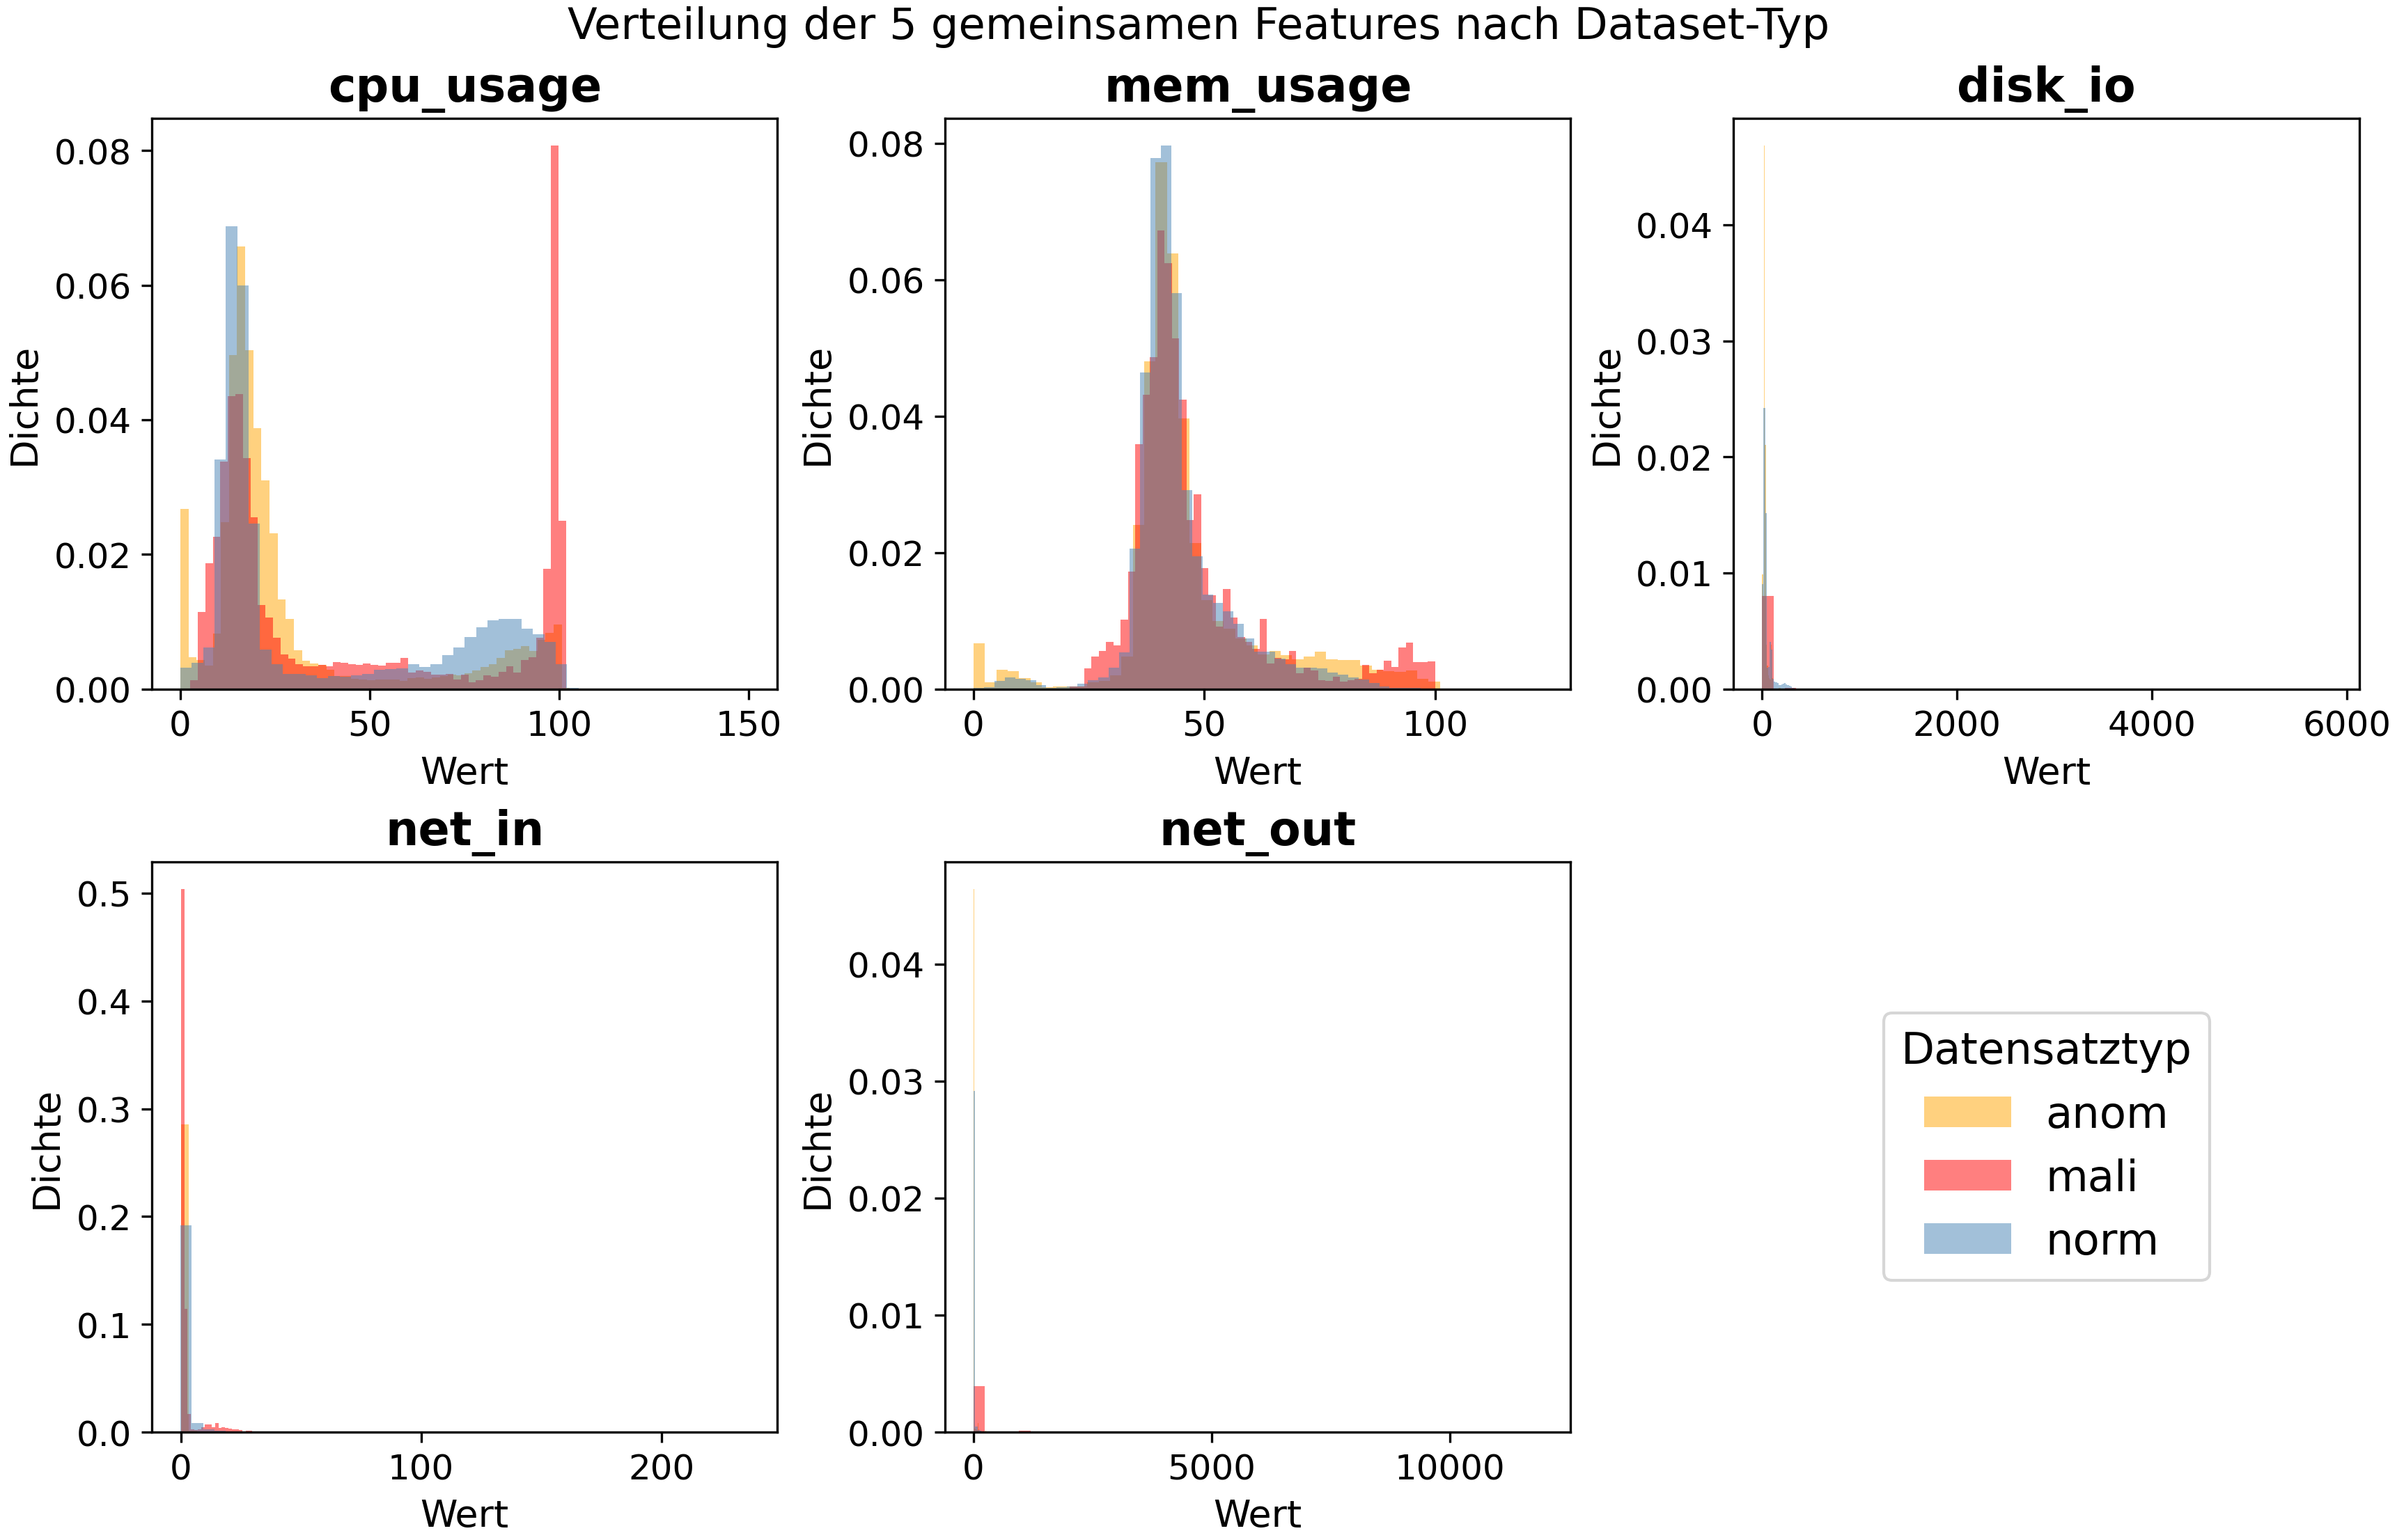
\includegraphics[width=0.95\textwidth]{../docs/feature_distributions}
  \caption{Verteilung der fünf universellen Features nach Datensatztyp (anom, mali, norm).}
  \label{fig:feat_dist}
\end{figure}

\subsection{Leakage-Vermeidung und Split-Strategie}

Für eine leakage-sichere Evaluation werden die Daten in drei disjunkte Teilmengen aufgeteilt. Als Gruppenkennung dient die Kombination aus \texttt{dataset\_type} und \texttt{scenario\_id} (\texttt{group\_id}), sodass kein Szenario in mehr als einer Teilmenge erscheint. Die Aufteilung erfolgt in zwei Stufen mit \texttt{GroupShuffleSplit}~\cite{roberts2017cross}: In einem ersten äußeren Schritt werden ca.\ 20~\% der Gruppen als Testset abgetrennt. In einem zweiten inneren Schritt werden aus dem verbleibenden Pool ca.\ 20~\% als Validierungsset reserviert. Das Trainingsset dient ausschließlich dem Modelltraining und der Imputation. Das Validierungsset wird für Early Stopping und die Threshold-Wahl verwendet, und das Testset wird ausschließlich zur finalen Evaluation eingesetzt. Die Nicht-Überlappung aller drei Splits nach Gruppenkennung wurde artefaktseitig verifiziert (\texttt{docs/split\_assignments.csv}). Beobachtungen innerhalb desselben Szenarios sind strukturell korreliert, sodass eine zufällige Aufteilung ohne Berücksichtigung dieser Gruppenstruktur die Trennleistung im Test systematisch überschätzen würde.

Tabelle~\ref{tab:split} fasst die resultierenden Teilmengen zusammen.

\begin{table}[htb]
  \centering
  \caption{Gruppenbasierter Train/Validation/Test-Split (\texttt{random\_state=42})}
  \label{tab:split}
  \begin{tabular}{lrrrr}
    \hline
    \textbf{Split} & \textbf{Cases} & \textbf{Gruppen} & \textbf{Positiv} & \textbf{Negativ} \\
    \hline
    Train      & 793 & 28 & 122 & 671 \\
    Validation & 206 &  8 &  53 & 153 \\
    Test       & 253 &  9 &  48 & 205 \\
    \hline
    \textbf{Gesamt} & \textbf{1\,252} & \textbf{45} & \textbf{223} & \textbf{1\,029} \\
    \hline
  \end{tabular}
\end{table}

Das Klassenungleichgewicht im Trainingsset beträgt 5{,}50:1 (negativ zu positiv, 671~vs.\ 122~Cases).

% ---------------------------------------------------------------------------
\section{Metrikbasierte Baseline}
% ---------------------------------------------------------------------------

\subsection{Modellwahl und Hyperparameter}

Als Baseline-Modell für den metrikbasierten Anomalie-Detektor wird XGBoost~\cite{chen2016xgboost} eingesetzt. XGBoost implementiert Gradient Boosting über Entscheidungsbäume und ist durch die \texttt{hist}-Methode (histogrammbasiertes Split-Finding) auch für größere Datensätze effizient anwendbar. Für tabellarisch strukturierte Daten mit gemischten Skalen stellt XGBoost eine gut validierte Wahl dar.

Als Optimierungsmetrik wird der Wert der Fläche unter der Precision-Recall-Kurve (\emph{AUCPR}) gewählt. Bei stark unbalancierten Klassifikationsproblemen ist AUCPR gegenüber dem ROC-AUC informativer, da Letzterer die Leistung im negativen Regime übergewichtet~\cite{davis2006relationship,saito2015precision}. Das vorliegende Klassenungleichgewicht im Trainingsset von annähernd 5{,}50:1 entspricht diesem Szenario~\cite{hegarcia2009learning}.

Das Klassenungleichgewicht wird in der XGBoost-Verlustfunktion über den Hyperparameter \texttt{scale\_pos\_weight} berücksichtigt. Der Wert von~5{,}50 wird ausschließlich aus der Trainingsverteilung berechnet (671 negative vs.\ 122 positive Trainingsfälle). Als Optimierungsmetrik dient AUCPR. Early Stopping ist mit 20 Runden aktiviert. Die Überwachungsmetrik wird dabei ausschließlich auf dem Validierungsset berechnet. Der Operating-Threshold wird als höchster Validierungsschwellenwert gewählt, der auf dem Validierungsset eine Recall-Rate von mindestens 0{,}95 erzielt. Die so bestimmte Schwelle wird unverändert auf das Testset angewendet.

\begin{table}[htb]
  \centering
  \caption{XGBoost-Hyperparameter}
  \label{tab:xgb_params}
  \begin{tabular}{ll}
    \hline
    \textbf{Parameter} & \textbf{Wert} \\
    \hline
    \texttt{tree\_method}      & \texttt{hist} \\
    \texttt{eval\_metric}      & \texttt{aucpr} \\
    \texttt{scale\_pos\_weight} & 5{,}50 \\
    \texttt{random\_state}     & 42 \\
    Early Stopping             & aktiv (Überwachung auf Validierungsset) \\
    \hline
  \end{tabular}
\end{table}

\subsection{Schema-Leakage, Feature-Reduktion und Case-Level-Aggregation}

Eine direkte Verwendung der vollständigen kanonischen 34-Feature-Matrix würde ein gravierendes Datenleck-Problem erzeugen. Die 29 typspezifischen Features sind strukturell in bestimmten Typen als \texttt{NaN} belegt: Ein Modell, das auf dieser Matrix trainiert, kann das bloße Muster fehlender Werte zur Bestimmung des Datensatztyps und damit der Klassenzugehörigkeit nutzen, noch bevor es ein inhaltliches Signal verarbeitet hat. Kaufman~et~al.~\cite{kaufman2012leakage} bezeichnen diese Konstellation als \emph{Target Leakage}, da die Feature-Struktur die Zielvariable implizit enkodiert.

Die Metrik-Baseline wird daher ausschließlich auf den fünf universellen Features trainiert und evaluiert (vgl. Abschnitt~\ref{sec:features}). Diese sind in allen drei Datensatztypen vorhanden und tragen kein typspezifisches Strukturmuster.

Um Zeitreiheninformationen auf Case-Ebene nutzbar zu machen, werden die Rohmessreihen jeder Case pro Metrik zu fünf statistischen Aggregaten verdichtet: Mittelwert (\texttt{mean}), Maximum (\texttt{max}), Standardabweichung (\texttt{std}), 95.~Perzentil (\texttt{p95}) und linearer Trend (\texttt{slope}). Dies ergibt eine Feature-Matrix mit $5 \times 5 = 25$~Case-Level-Features. Das XGBoost-Modell wird direkt auf dieser Case-Level-Feature-Matrix trainiert. Ein separater Row-Level-Klassifikationsschritt entfällt. Fehlende Feature-Werte werden durch den auf dem Trainingsset berechneten Median imputiert (kein Leakage).

\subsection{Ergebnisse der Metrik-Baseline}
\label{sec:baseline}

\begin{table}[htb]
  \centering
  \caption{Ergebnisse der Metrik-Baseline (XGBoost, Case-Ebene, 25~Features, Testset $n=253$)}
  \label{tab:baseline_results}
  \begin{tabular}{ll}
    \hline
    \textbf{Metrik} & \textbf{Wert} \\
    \hline
    Average Precision (AP)                               & 0{,}2652 \\
    Threshold (Val-Recall$_{\text{mali}}$ $\geq$ 0{,}95) & 0{,}0258 \\
    Recall$_{\text{mali}}$ @ Threshold                   & 1{,}0000 \\
    Precision @ Threshold                                & 0{,}1897 \\
    F1-Maß @ Threshold                                   & 0{,}3189 \\
    FPR$_{\text{total}}$                                 & 1{,}0000 (205 / 205 Negative) \\
    FPR$_{\text{anom}}$                                  & 1{,}0000 (76 / 76) \\
    FPR$_{\text{norm}}$                                  & 1{,}0000 (129 / 129) \\
    TP\,/\,FP\,/\,TN\,/\,FN                             & 48\,/\,205\,/\,0\,/\,0 \\
    \hline
  \end{tabular}
\end{table}

Tabelle~\ref{tab:baseline_results} fasst die Ergebnisse zusammen. Der XGBoost-Detektor erkennt auf Case-Ebene alle 48 positiven Test-Cases
(Recall$_{\text{mali}}$ = 1{,}0000), klassifiziert aber gleichzeitig alle 205 negativen Cases als positiv (FPR$_{\text{total}}$ = 1{,}0000, TN~=~0). Die Metrik-Komponente ist auf diesem Benchmark \emph{nicht selektiv}: Sie kann nicht zwischen mali- und anom- und norm-Cases unterscheiden, weil viele technische Anomalien und Normalszenarien ähnlich hohe Metrik-Aggregate wie Malware-Aktivitäten aufweisen. Der niedrige Threshold von~0{,}0258 (bestimmt auf dem Validierungsset) markiert alle Test-Cases als metrisch auffällig.

Abbildung~\ref{fig:pr_baseline} zeigt die zugehörige Precision-Recall-Kurve. Abbildung~\ref{fig:feat_imp} visualisiert die Feature-Importances des trainierten Modells nach dem Gain-Kriterium.

\begin{figure}[htb]
  \centering
  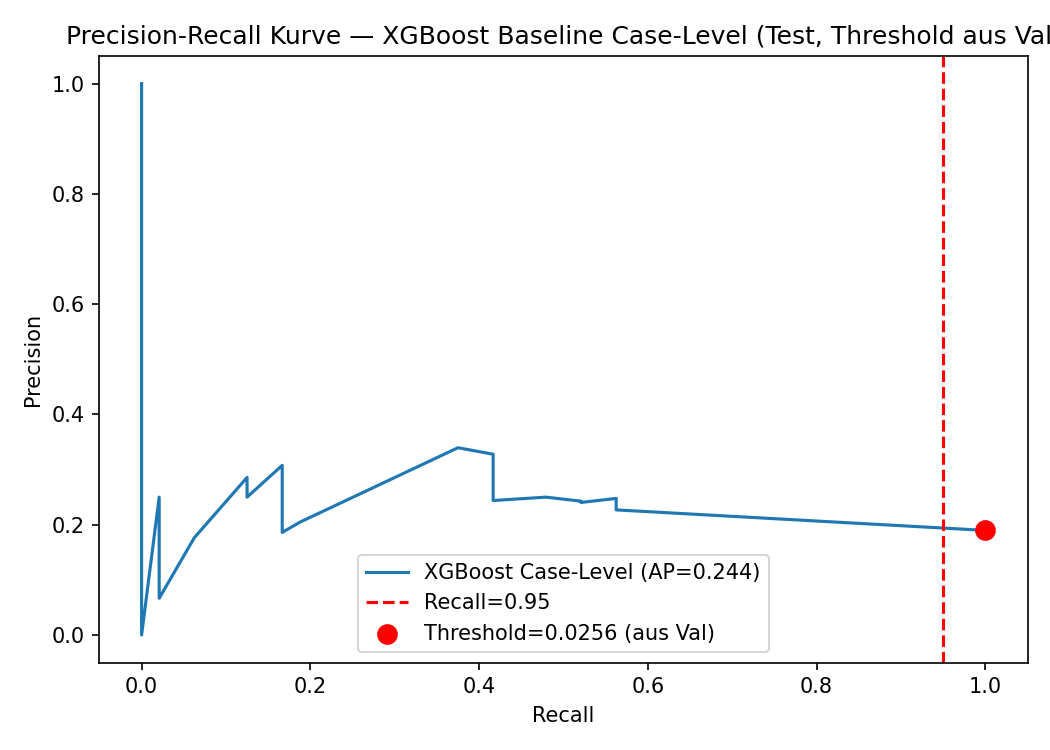
\includegraphics[width=0.78\textwidth]{../docs/pr_curve_baseline}
  \caption{Precision-Recall-Kurve der Metrik-Baseline (AP = 0{,}2652, Case-Ebene). Der markierte Punkt entspricht dem Threshold~0{,}026 (aus Validierungsset) bei Recall$_{\text{mali}}$ = 1{,}0000.}
  \label{fig:pr_baseline}
\end{figure}

\begin{figure}[htb]
  \centering
  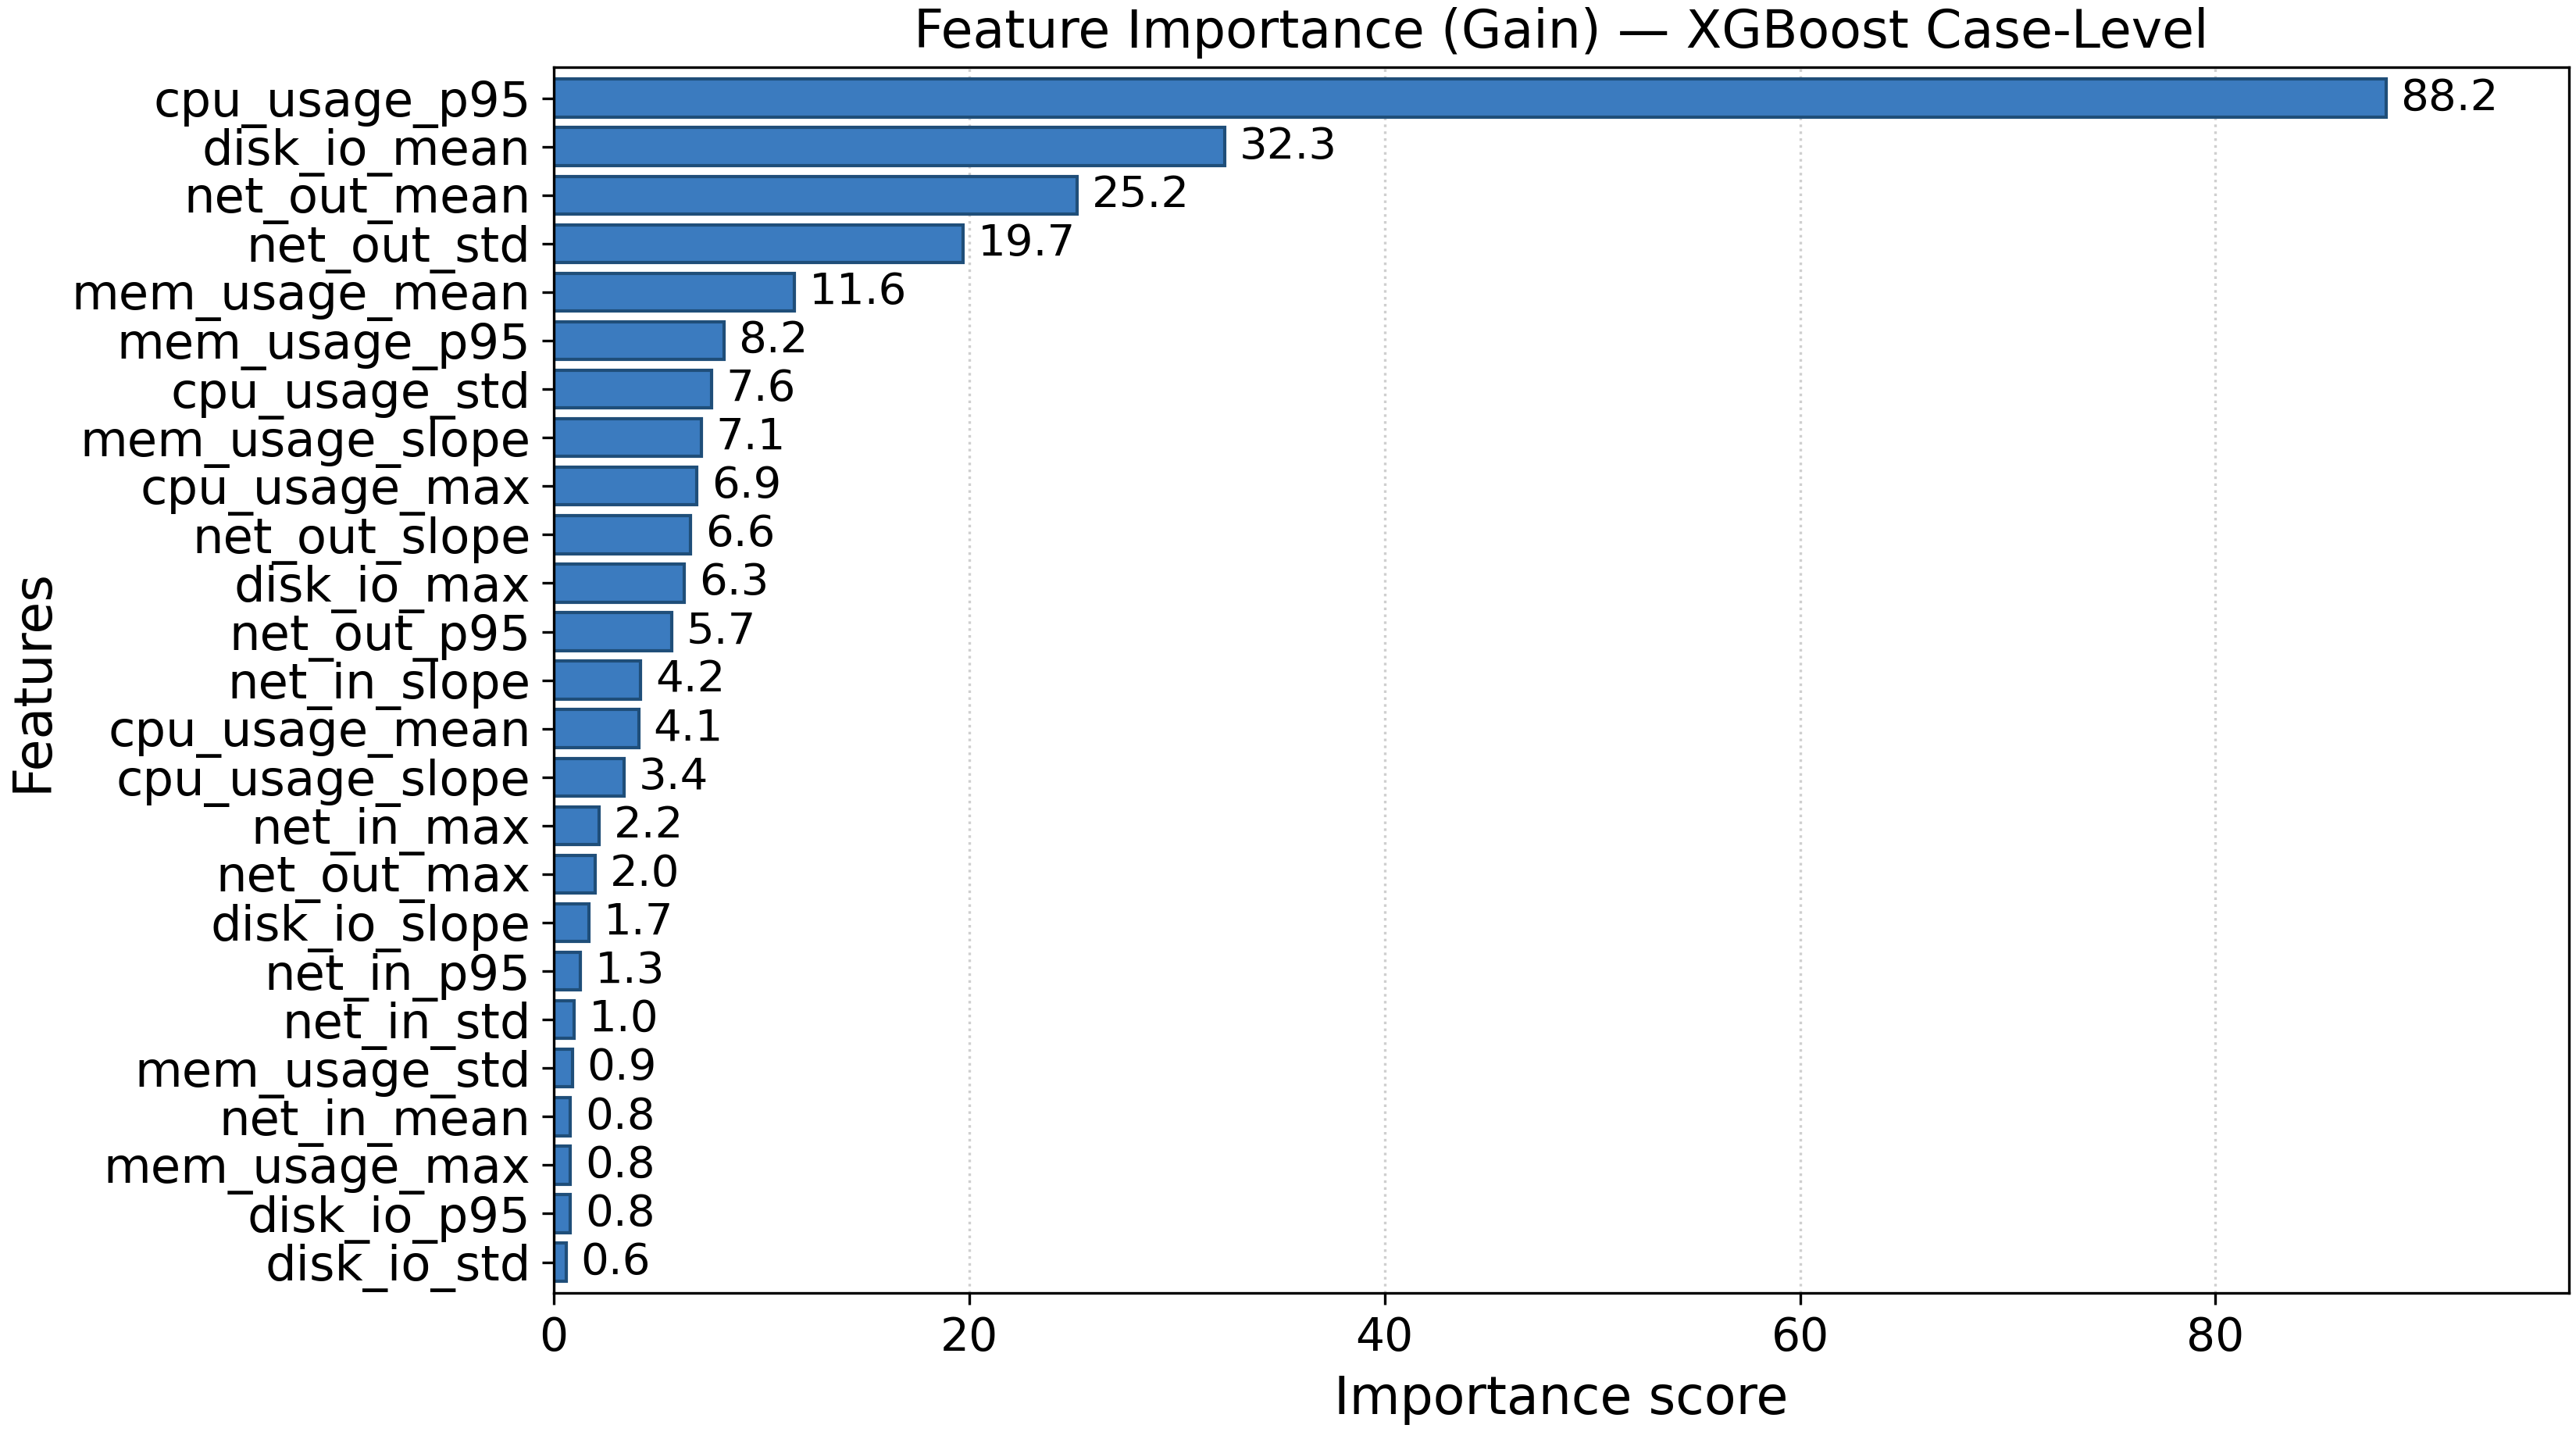
\includegraphics[width=0.78\textwidth]{../docs/feature_importance_baseline}
  \caption{Feature-Importances (Gain) des XGBoost-Modells auf den 25~Case-Level-Features (5~Metriken $\times$ 5~Aggregationen).}
  \label{fig:feat_imp}
\end{figure}

Die Metrik-Baseline ist auf Case-Ebene zwar vollständig sensitiv (Recall$_{\text{mali}}$ = 1{,}0000), aber nicht selektiv (FPR$_{\text{total}}$ = 1{,}0000). Dieser Befund motiviert die in Abschnitt~\ref{sec:log} beschriebene log-basierte Komponente.

% ---------------------------------------------------------------------------
\section{Log-basierte Verifikation}
\label{sec:log}
% ---------------------------------------------------------------------------

\subsection{Log-Daten auf Case-Ebene}

Für jeden der 1\,252 Cases liegt eine zugehörige Log-Datei vor. Die Log-Analyse operiert analog zur metrischen Analyse auf Case-Ebene: Jede Log-Datei wird als ein einzelnes Dokument behandelt, dem genau ein binäres Label zugewiesen ist. Log-Daten enthalten qualitative Textinformationen über Systemereignisse, Fehlermeldungen und Prozessabläufe, die Metriken allein nicht abbilden können. He~et~al.~\cite{he2021survey} zeigen in ihrer Übersicht, dass automatisierte Log-Analyse ein etabliertes Werkzeug im Reliability Engineering ist und textbasierte Merkmale relevante Signale für die Anomalieerkennung liefern.

Von 1\,252 Cases des Gesamtdatensatzes entfallen nach dem gruppenbasierten dreistufigen Split 793~Fälle auf das Trainingsset, 206~auf das Validierungsset und 253~auf das Testset. Im Testset befinden sich 48~positive (mali), 76~anom und 129~norm-Cases.

\subsection{Log-Normalisierung}

Bevor die Log-Texte vektorisiert werden, werden synthetische Artefakte durch generische Token-Platzhalter ersetzt. Dieser Schritt ist deterministisch und regelbasiert. Er verursacht kein Datenleck, da er unabhängig von den Labels ist und auf alle Splits gleichartig angewendet wird.

\begin{table}[htb]
  \centering
  \caption{Regelbasierte Log-Normalisierung: Ersetzte Muster und ihre Token-Platzhalter}
  \label{tab:log_norm}
  \resizebox{\linewidth}{!}{%
  \begin{tabular}{lll}
    \hline
    \textbf{Muster} & \textbf{Token} & \textbf{Beispiel} \\
    \hline
    UUIDs                        & \texttt{TOKEN\_ID}   & \texttt{550e8400-\ldots} $\rightarrow$ \texttt{TOKEN\_ID} \\
    Nginx-Zeitstempel            & \texttt{TOKEN\_TIME} & \texttt{[20/Aug/2025:08:01:10 +0000]} $\rightarrow$ \texttt{TOKEN\_TIME} \\
    Syslog-Zeitstempel           & \texttt{TOKEN\_TIME} & \texttt{Aug 15 10:00:05} $\rightarrow$ \texttt{TOKEN\_TIME} \\
    ISO-Zeitstempel (mit Zeit)   & \texttt{TOKEN\_TIME} & \texttt{2024-01-12T13:45:22Z} $\rightarrow$ \texttt{TOKEN\_TIME} \\
    ISO-Datum                    & \texttt{TOKEN\_DATE} & \texttt{2024-01-12} $\rightarrow$ \texttt{TOKEN\_DATE} \\
    Uhrzeiten                    & \texttt{TOKEN\_TIME} & \texttt{13:45:22} $\rightarrow$ \texttt{TOKEN\_TIME} \\
    IPv4-Adressen                & \texttt{TOKEN\_IP}   & \texttt{192.168.1.10} $\rightarrow$ \texttt{TOKEN\_IP} \\
    PIDs (in \texttt{[]})        & \texttt{TOKEN\_PID}  & \texttt{sshd[11532]} $\rightarrow$ \texttt{sshd[TOKEN\_PID]} \\
    Ports                        & \texttt{TOKEN\_PORT} & \texttt{port 54321} $\rightarrow$ \texttt{port TOKEN\_PORT} \\
    Isolierte Zahlen             & \texttt{TOKEN\_NUM}  & \texttt{retry 3} $\rightarrow$ \texttt{retry TOKEN\_NUM} \\
    \hline
  \end{tabular}}%
\end{table}

Sicherheitsrelevante semantische Information bleibt erhalten: Prozessnamen (\texttt{sshd}, \texttt{CRON}, \texttt{wget}, \texttt{curl}, \texttt{bash}), Aktionen (\texttt{Accepted}, \texttt{Failed}, \texttt{CMD}), Pfade, Domains und Protokollbezeichner werden nicht verändert. Es sei darauf hingewiesen, dass einige dieser Terme, etwa \texttt{sshd}, \texttt{cron} oder \texttt{bash}, in regulärem Systembetrieb generisch auftreten können. Sie sind Teil der vordefinierten Security-Keyword-Liste, nicht per se Angriffshinweise. Die Motivation dieser Normalisierung besteht darin, dass synthetische Artefakte wie Zeitstempel und IP-Adressen in einem Benchmarkdatensatz zufällig variieren und kein semantisches Signal tragen. Das TF-IDF-Modell soll stattdessen auf dem inhaltlich relevanten Vokabular trainiert werden.

\subsection{TF-IDF-Vektorisierung}

Die Textrepräsentation erfolgt mit \emph{Term Frequency~-- Inverse Document Frequency} (TF-IDF). TF-IDF gewichtet Terme nach ihrer Auftretenshäufigkeit im Dokument, normiert dabei jedoch durch die Häufigkeit über alle Dokumente hinweg, sodass häufige, wenig diskriminierende Terme abgewertet werden. TF-IDF stellt eine interpretierbare und effizient trainierbare Baseline dar. Fortgeschrittenere Ansätze wie Log-Parser oder Embedding-Methoden wurden im Rahmen dieser Arbeit nicht untersucht und bilden eine naheliegende Erweiterung. Für Log-Daten ist die TF-IDF-Gewichtung dennoch sinnvoll, da generische Systemereignisse (z.\,B. regelmäßige Statusmeldungen) häufig auftreten, aber geringe Trennkraft besitzen~\cite{he2021survey}.

\begin{table}[htb]
  \centering
  \caption{TF-IDF-Konfiguration}
  \label{tab:tfidf_params}
  \begin{tabular}{ll}
    \hline
    \textbf{Parameter} & \textbf{Wert} \\
    \hline
    \texttt{max\_features}  & 10\,000 \\
    \texttt{ngram\_range}   & (1,\,2) \\
    \texttt{sublinear\_tf}  & \texttt{True} \\
    \texttt{min\_df}        & 2 \\
    Fit                     & ausschließlich auf Trainingsfälle \\
    \hline
  \end{tabular}
\end{table}

Der Vektorisierer wird ausschließlich auf den 793~Trainingsfällen gefittet. Weder das Validierungs- noch das Test-Vokabular wird einbezogen~\cite{kaufman2012leakage}. Die Verwendung von Bigrammen erlaubt die Erfassung kurzer Wortfolgen, die in Log-Meldungen häufig als feste Phrasen auftreten. Der Parameter \texttt{ngram\_range} ist auf \texttt{(1,\,2)} gesetzt. Mit \texttt{sublinear\_tf=True} wird die rohe Termfrequenz durch ihren Logarithmus ersetzt, um sehr häufige Terme nicht unverhältnismäßig zu gewichten. Das resultierende Vokabular umfasst 10\,000~Terme. Die Trainings-, Validierungs- und Testmatrix haben die Dimension $(793 \times 10\,000)$, $(206 \times 10\,000)$ bzw. $(253 \times 10\,000)$.

\subsection{Logistische Regression}

Auf der TF-IDF-Matrix wird eine logistische Regression trainiert. Lineare Klassifikatoren auf sparse hochdimensionalen Textmatrizen sind für diese Problemklasse eine gut erprobte Wahl. Die Implementierung erfolgt über die logistische Regression aus scikit-learn~\cite{pedregosa2011scikit}. Der \texttt{lbfgs}-Solver ist auf mittelgroßen Datensätzen numerisch stabil und effizient einsetzbar. Das Klassenungleichgewicht (Trainingsverhältnis $\approx$~5{,}50:1) wird durch \texttt{class\_weight=`balanced'} ausgeglichen, das die Verlustfunktion proportional zu den Klassengrößen gewichtet.

\begin{table}[htb]
  \centering
  \caption{Hyperparameter der logistischen Regression}
  \label{tab:logreg_params}
  \begin{tabular}{ll}
    \hline
    \textbf{Parameter} & \textbf{Wert} \\
    \hline
    \texttt{class\_weight} & \texttt{balanced} \\
    \texttt{solver}        & \texttt{lbfgs} \\
    \texttt{C}             & 1{,}0 \\
    \texttt{max\_iter}     & 1\,000 \\
    \hline
  \end{tabular}
\end{table}

Abbildung~\ref{fig:tfidf_feat} visualisiert die 20~einflussreichsten Terme des Modells nach Koeffizientengröße, getrennt nach positiv und negativ gewichteten Termen.

\begin{figure}[htb]
  \centering
  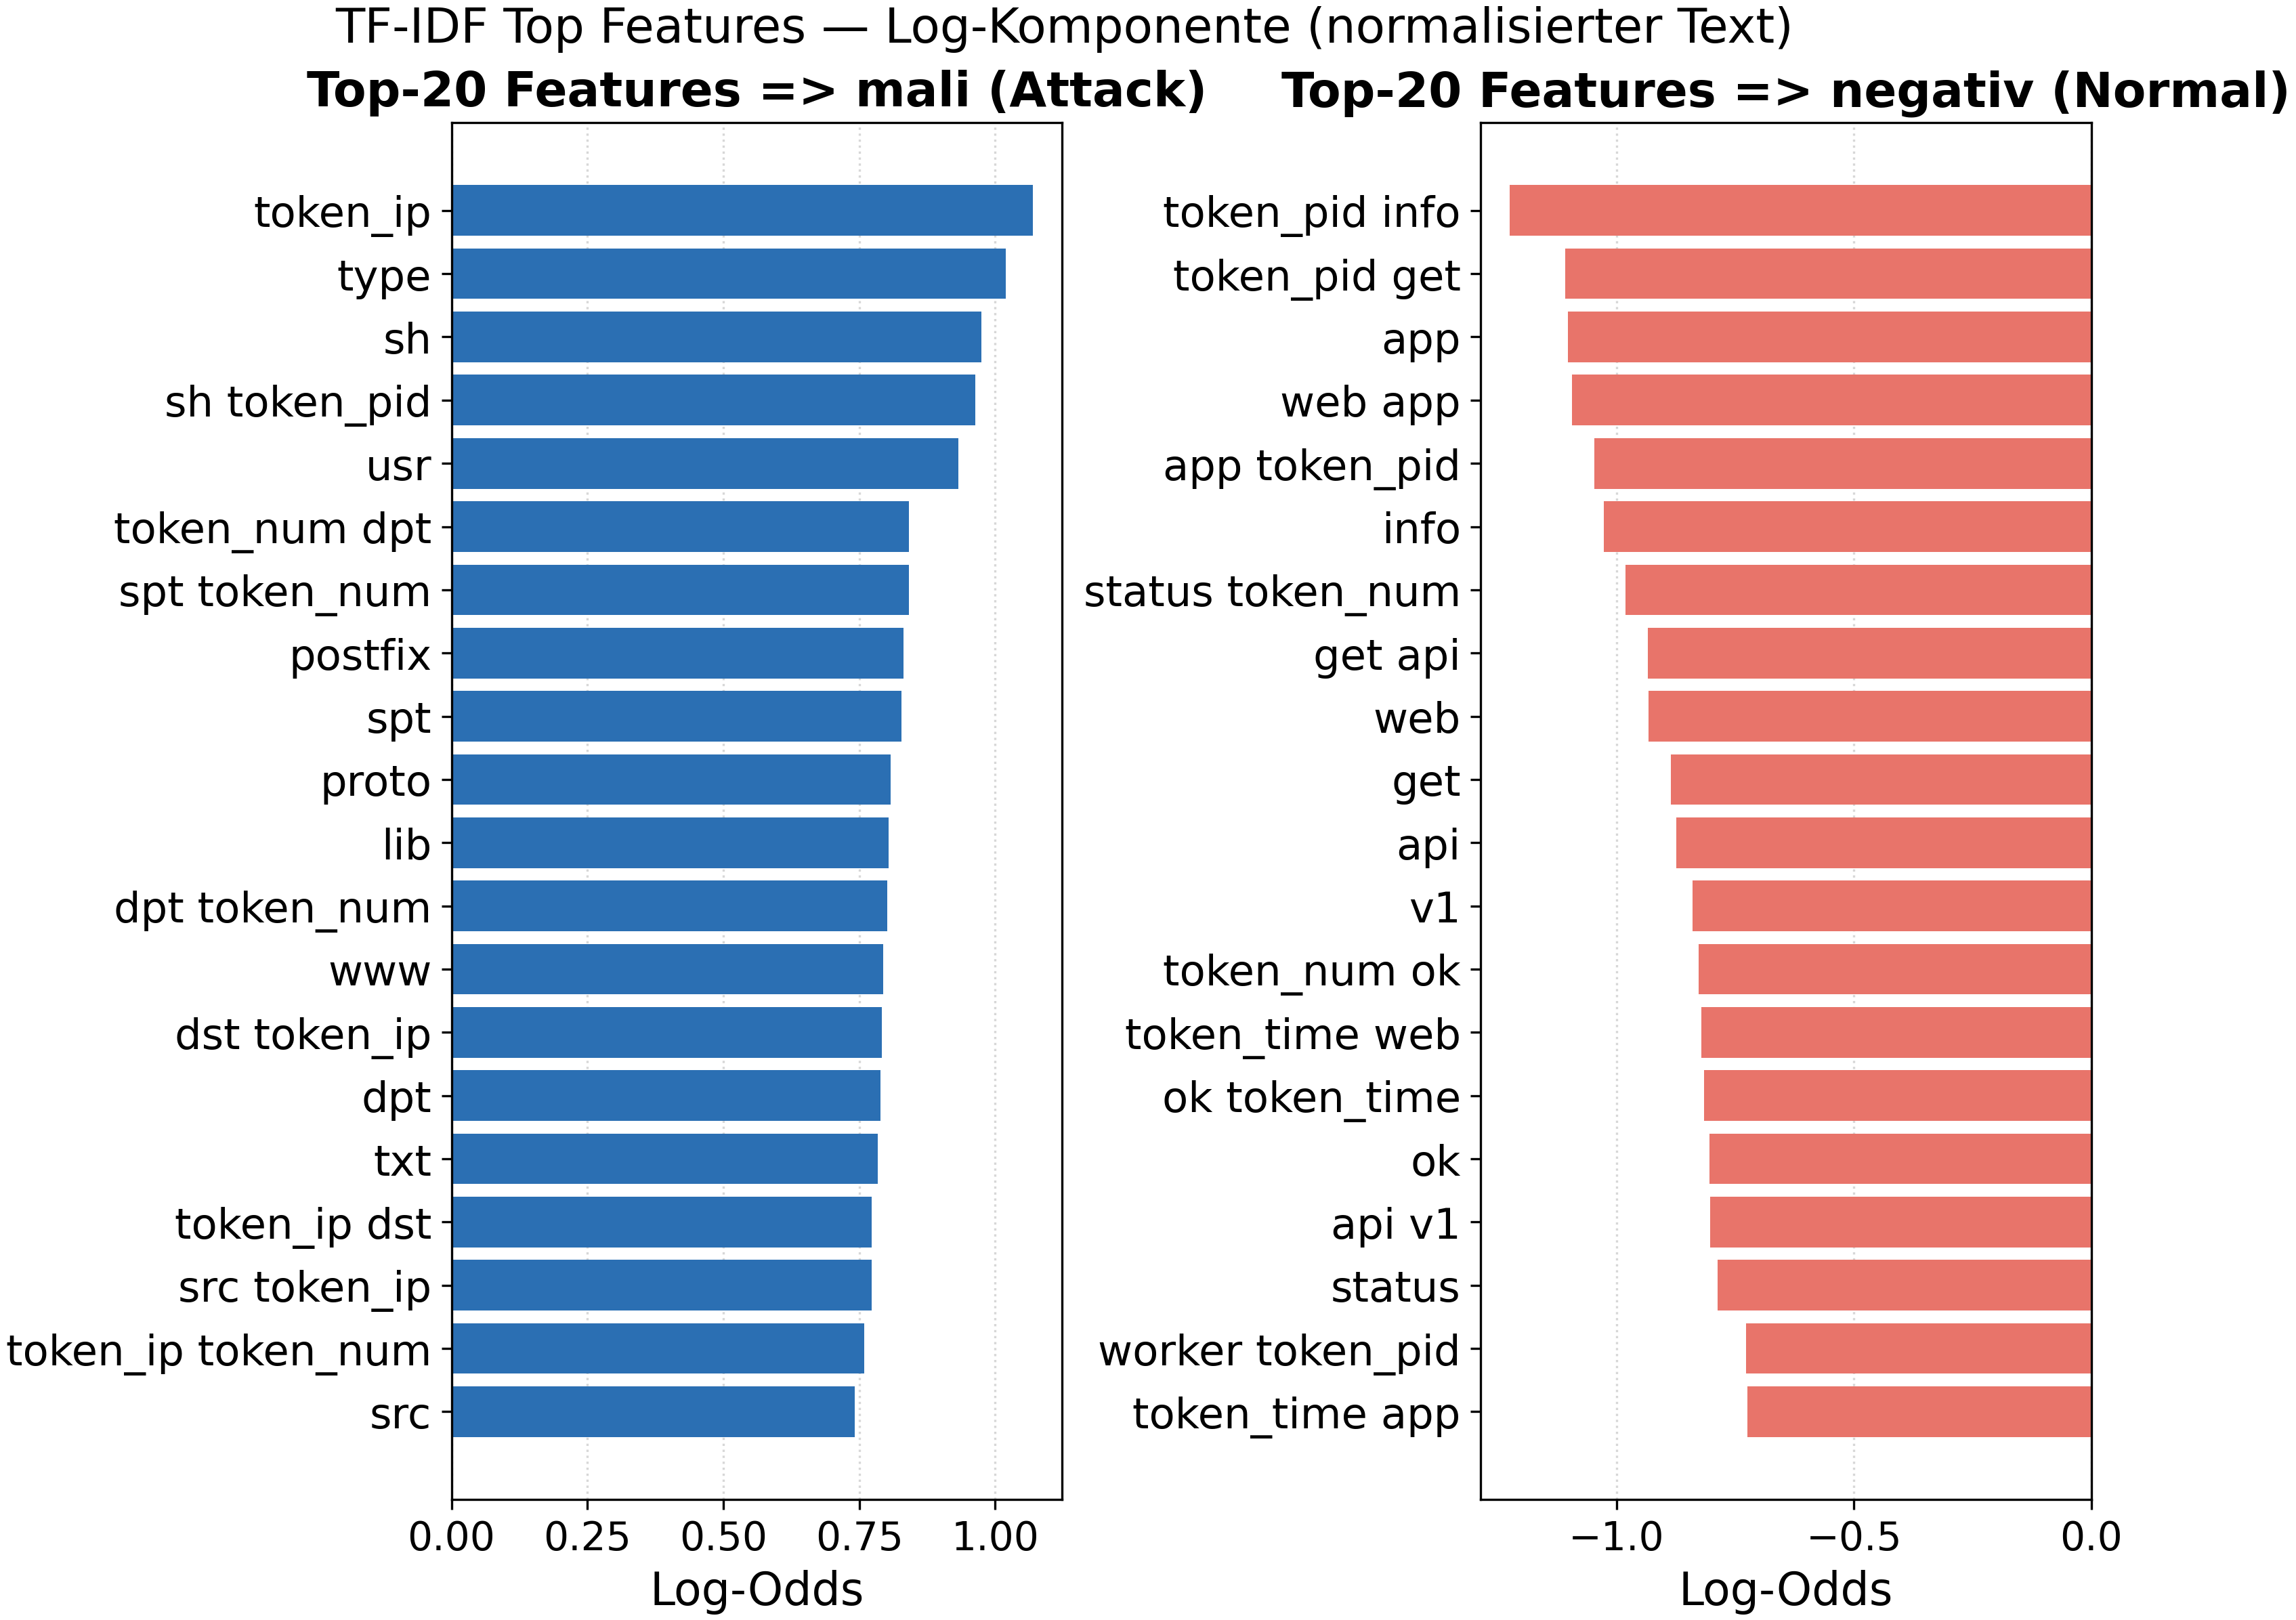
\includegraphics[width=\textwidth]{../docs/tfidf_top_features}
  \caption{Top-20 TF-IDF-Terme nach Koeffizientengröße. Positiv gewichtete Terme sind stärker mit malignen Cases assoziiert. Negativ gewichtete Terme treten häufiger in benignen Cases auf.}
  \label{fig:tfidf_feat}
\end{figure}

Der Operating-Threshold der Log-Komponente wird auf dem Validierungsset bestimmt: Es wird der höchste Validierungsschwellenwert gewählt, der auf dem Validierungsset eine Recall$_{\text{mali}}$-Rate von mindestens 0{,}95 erzielt. Die so bestimmte Schwelle (0{,}164) wird anschließend unverändert auf das Testset angewendet.

\subsection{Ergebnisse der Log-Komponente}

\begin{table}[htb]
  \centering
  \caption{Ergebnisse der Log-Komponente (TF-IDF + LogReg, normalisiert, Case-Ebene, Testset $n=253$)}
  \label{tab:log_results}
  \begin{tabular}{ll}
    \hline
    \textbf{Metrik} & \textbf{Wert} \\
    \hline
    Average Precision (AP)                               & 0{,}6548 \\
    Threshold (Val-Recall$_{\text{mali}}$ $\geq$ 0{,}95) & 0{,}1641 \\
    Recall$_{\text{mali}}$ @ Threshold                   & 0{,}9375 \\
    Precision @ Threshold                                & 0{,}4639 \\
    F1-Maß @ Threshold                                   & 0{,}6207 \\
    FPR$_{\text{total}}$                                 & 0{,}2537 (52 / 205 Negative) \\
    FPR$_{\text{anom}}$                                  & 0{,}2368 (18 / 76) \\
    FPR$_{\text{norm}}$                                  & 0{,}2636 (34 / 129) \\
    TP\,/\,FP\,/\,TN\,/\,FN                             & 45\,/\,52\,/\,153\,/\,3 \\
    \hline
  \end{tabular}
\end{table}

Tabelle~\ref{tab:log_results} zeigt die Ergebnisse der Log-Komponente. Gegenüber der nicht-selektiven Metrik-Baseline (FPR$_{\text{total}}$ = 1{,}0000) sinkt die FPR auf 0{,}2537. Die Log-Komponente ist die einzige Variante mit echter Selektivität. Der Test-Recall$_{\text{mali}}$ beträgt 0{,}9375 (45 von 48 positiven Cases erkannt, 3~FN), womit die angestrebte Schwelle von 0{,}95 knapp verfehlt wird. Getrennt nach Negativtypen ergeben sich FPR$_{\text{anom}}$ = 0{,}2368 und FPR$_{\text{norm}}$ = 0{,}2636. Abbildung~\ref{fig:pr_log} zeigt die zugehörige PR-Kurve. Ein direkter AP-Vergleich mit der Metrik-Baseline ist nun auf gleicher Granularität (Case-Ebene, $n=253$) möglich.

\begin{figure}[htb]
  \centering
  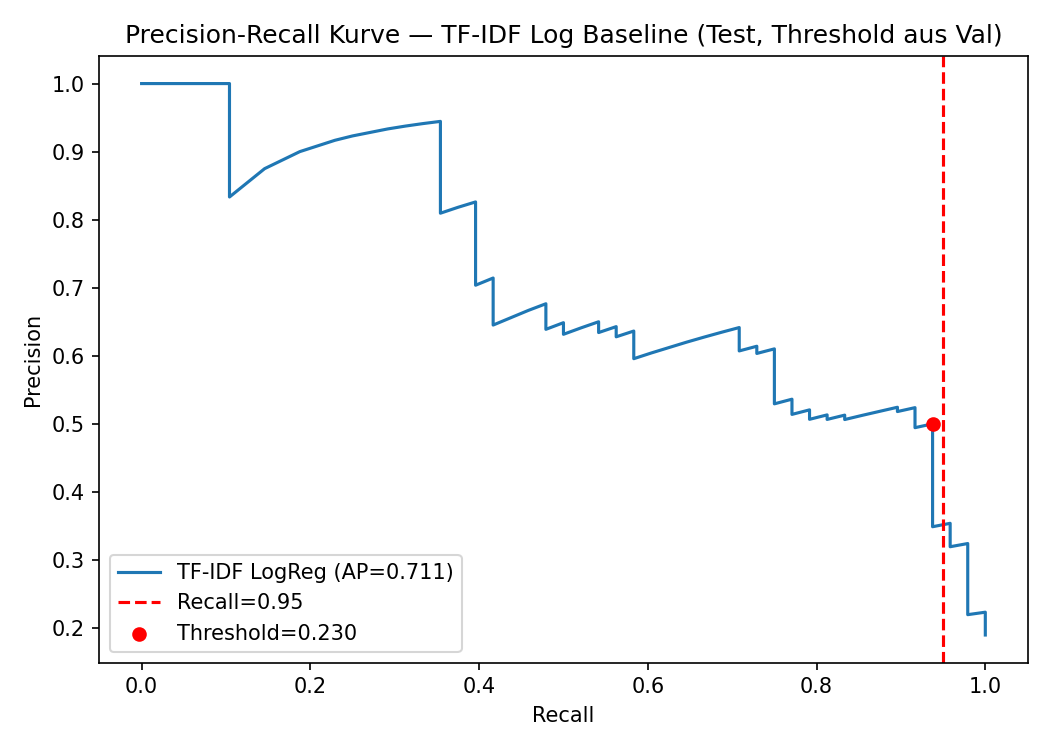
\includegraphics[width=0.78\textwidth]{../docs/pr_curve_log}
  \caption{Precision-Recall-Kurve der Log-Komponente (AP = 0{,}6548, Case-Ebene). Der markierte Punkt entspricht dem Threshold~0{,}164 (aus Validierungsset) bei Recall$_{\text{mali}}$ = 0{,}9375.}
  \label{fig:pr_log}
\end{figure}

\subsection{Threshold-Sensitivity-Analyse}
\label{sec:sensitivity}

Zur methodischen Absicherung der Threshold-Wahl wurde eine Sensitivity-Analyse für die Log-Komponente durchgeführt. Es wurden vier Validierungs-Recall-Ziele untersucht: 0{,}95, 0{,}975, 0{,}99 und 1{,}00. Für jedes Ziel wurde der höchste Validierungsschwellenwert bestimmt, der auf dem Validierungsset das jeweilige Recall-Ziel erfüllt. Dieser Threshold wurde anschließend unverändert auf das Testset angewendet. Die resultierenden Testmetriken dienen ausschließlich der Auswertung und wurden zu keinem Zeitpunkt für die Threshold-Auswahl herangezogen. Eine testbasierte Nachoptimierung wurde bewusst nicht vorgenommen.

\begin{table}[htb]
  \centering
  \caption{Threshold-Sensitivity der Log-Komponente (Case-Ebene, Threshold und Val-Recall aus Validierungsset)}
  \label{tab:sensitivity}
  \resizebox{\linewidth}{!}{%
  \begin{tabular}{lllllllll}
    \hline
    \textbf{Val-Recall-Ziel} & \textbf{Threshold} & \textbf{Val-Recall} & \textbf{Test-Recall} & \textbf{Test-FPR} & \textbf{FPR\textsubscript{anom}} & \textbf{FPR\textsubscript{norm}} & \textbf{Precision} & \textbf{F1} \\
    \hline
    0{,}950 & 0{,}1641 & 0{,}9623 & 0{,}9375 & 0{,}2537 & 0{,}2368 & 0{,}2636 & 0{,}4639 & 0{,}6207 \\
    0{,}975 & 0{,}1228 & 1{,}0000 & 0{,}9375 & 0{,}3512 & 0{,}4079 & 0{,}3178 & 0{,}3846 & 0{,}5455 \\
    0{,}990 & 0{,}1228 & 1{,}0000 & 0{,}9375 & 0{,}3512 & 0{,}4079 & 0{,}3178 & 0{,}3846 & 0{,}5455 \\
    1{,}000 & 0{,}1228 & 1{,}0000 & 0{,}9375 & 0{,}3512 & 0{,}4079 & 0{,}3178 & 0{,}3846 & 0{,}5455 \\
    \hline
  \end{tabular}}%
\end{table}

Tabelle~\ref{tab:sensitivity} zeigt das zentrale Ergebnis: Bei allen vier Recall-Zielen bleibt der Test-Recall konstant bei 0{,}9375. Höhere Validierungsziele führen zu einem niedrigeren Threshold und einer höheren FPR$_{\text{total}}$ (von 0{,}2537 auf 0{,}3512), ohne den Test-Recall zu verbessern. Bei dem auf Validation ausgewählten Threshold bleiben die drei False-Negative-Cases unterhalb der Entscheidungsgrenze. Eine niedrigere Schwelle könnte den Recall erhöhen, würde jedoch voraussichtlich zusätzliche False Positives erzeugen. Dieser Trade-off wird in der Threshold-Sensitivity sichtbar. Diese Limitation wird in Abschnitt~\ref{sec:limit} ausführlich diskutiert.

% ---------------------------------------------------------------------------
\section{Hybride Fusion und Evaluation}
% ---------------------------------------------------------------------------

\subsection{Fusion-Eingaben auf Case-Ebene}

Beide Komponenten liefern direkt Case-Level-Scores. Die Metrik-Komponente (Abschnitt~\ref{sec:baseline}) gibt pro Case einen Score $\hat{p}_{\text{metric}}$ aus, der mit dem Validierungsschwellenwert von~0{,}0258 in einen binären \texttt{metric\_trigger} umgewandelt wird. Die Log-Komponente (Abschnitt~\ref{sec:log}) gibt pro Case einen Log-Score $\hat{p}_{\text{log}}$ aus, der mit dem Validierungsschwellenwert von~0{,}164 in einen binären \texttt{log\_trigger} umgewandelt wird. Ein Row-Level-Aggregationsschritt ist nicht erforderlich, da das Metrik-Modell direkt auf Case-Level-Aggregaten trainiert wurde.

Im Testset von 253~Cases ergibt die metrische Klassifikation folgende Verteilung:

\begin{center}
  \texttt{metric\_trigger = 1}: 253~Cases (100~\%) \quad
  \texttt{metric\_trigger = 0}: 0~Cases
\end{center}

Dieser Befund ist zentral für die Interpretation der nachfolgenden Fusion und wird in Abschnitt~\ref{sec:degeneration} ausführlich diskutiert.

\subsection{AND-Gate-Fusion und Soft-Score}

Die Fusionsstufe kombiniert den binären Metriktrigger mit der log-basierten Klassifikation zu einem Alert-Signal. Es wurden zwei Fusionsstrategien untersucht:

\textbf{AND-Gate-Fusion (hart):}
\[
  \text{alert} = \mathbf{1}[\texttt{metric\_trigger} = 1 \;\wedge\; \texttt{log\_trigger} = 1]
\]
Das AND-Gate setzt einen Alert nur dann, wenn \emph{beide} Komponenten positiv entscheiden. Die konzeptuelle Motivation besteht darin, dass die Log-Komponente als Nachfilter wirkt: Nur Cases, die auch metrisch auffällig sind, werden auf Basis ihres Log-Kontexts abschließend bewertet~\cite{kittler1998combining}.

\textbf{Soft-Fusion:}
\[
  s_{\text{fusion}} = \hat{p}_{\text{metric}} \times \hat{p}_{\text{log}}
\]
Der Soft-Score ist das Produkt des metrischen Scores und des log-basierten Scores (vgl.~\cite{kittler1998combining}). Da beide Faktoren im Intervall $[0,\,1]$ liegen, gilt dies auch für $s_{\text{fusion}}$. Auf Basis dieses Scores kann eine vollständige PR-Kurve berechnet werden.

\subsection{Ablationsstudie}
\label{sec:ablation}

Tabelle~\ref{tab:ablation} stellt alle vier Systemvarianten auf Case-Ebene gegenüber. Abbildung~\ref{fig:ablation_pr} überlagert die PR-Kurven der Varianten mit kontinuierlichem Score. Abbildung~\ref{fig:fpr_comp} zeigt den FPR-Vergleich als Balkendiagramm.

\begin{table}[htb]
  \centering
  \caption{Ablationsergebnisse auf Case-Ebene (Testset: 253~Cases, 48~positiv / 205~negativ)}
  \label{tab:ablation}
  \resizebox{\linewidth}{!}{%
  \begin{tabular}{lcccccccc}
    \hline
    \textbf{Variante} & \textbf{Recall\textsubscript{mali}} & \textbf{Precision} & \textbf{F1} & \textbf{FPR\textsubscript{total}} & \textbf{FPR\textsubscript{anom}} & \textbf{FPR\textsubscript{norm}} & \textbf{AP} & \textbf{TP/FP/TN/FN} \\
    \hline
    Metrics-only & 1{,}0000 & 0{,}1897 & 0{,}3189 & 1{,}0000 & 1{,}0000 & 1{,}0000 & 0{,}2652 & 48/205/0/0 \\
    Log-only     & 0{,}9375 & 0{,}4639 & 0{,}6207 & 0{,}2537 & 0{,}2368 & 0{,}2636 & 0{,}6548 & 45/52/153/3 \\
    AND-Fusion   & 0{,}9375 & 0{,}4639 & 0{,}6207 & 0{,}2537 & 0{,}2368 & 0{,}2636 & --      & 45/52/153/3 \\
    Soft-Fusion  & 0{,}9375 & 0{,}4545 & 0{,}6122 & 0{,}2634 & 0{,}2500 & 0{,}2713 & 0{,}5553 & 45/54/151/3 \\
    \hline
    \multicolumn{9}{l}{Alle Varianten auf Case-Ebene, $n=253$. AP für AND-Fusion nicht anwendbar (binärer Trigger).} \\
  \end{tabular}}%
\end{table}

\begin{figure}[htb]
  \centering
  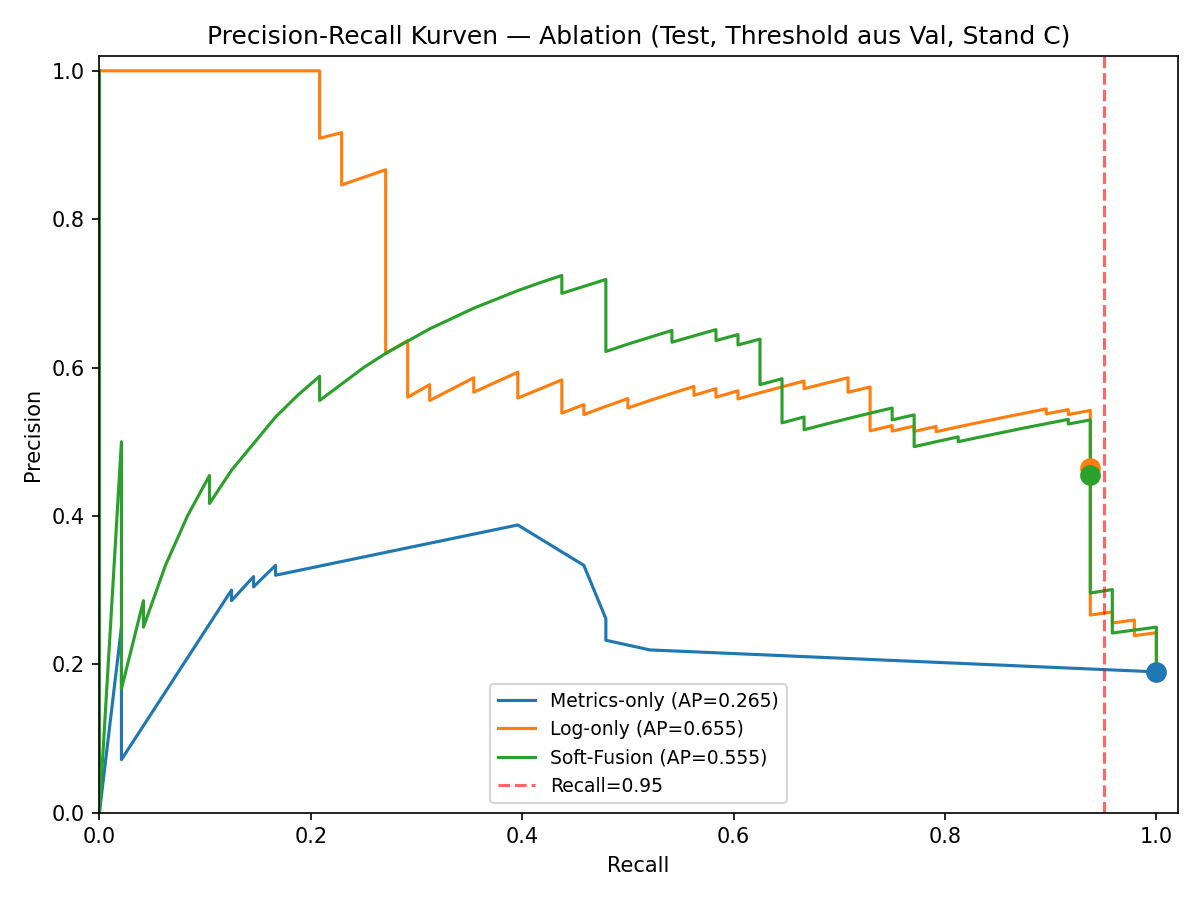
\includegraphics[width=0.78\textwidth]{../docs/pr_curve_ablation}
  \caption{Precision-Recall-Kurven der Case-Level-Ablation. Die Metrik-only-Kurve basiert auf dem Case-Level-Score des XGBoost-Modells. Die Soft-Fusion-Kurve basiert auf dem Produkt-Score $s = \hat{p}_{\text{metric}} \times \hat{p}_{\text{log}}$. AND-Fusion hat keinen kontinuierlichen Score und erscheint nicht als Kurve. Alle AP-Werte beziehen sich auf dieselbe Granularität (Case-Ebene, $n=253$).}
  \label{fig:ablation_pr}
\end{figure}

\begin{figure}[htb]
  \centering
  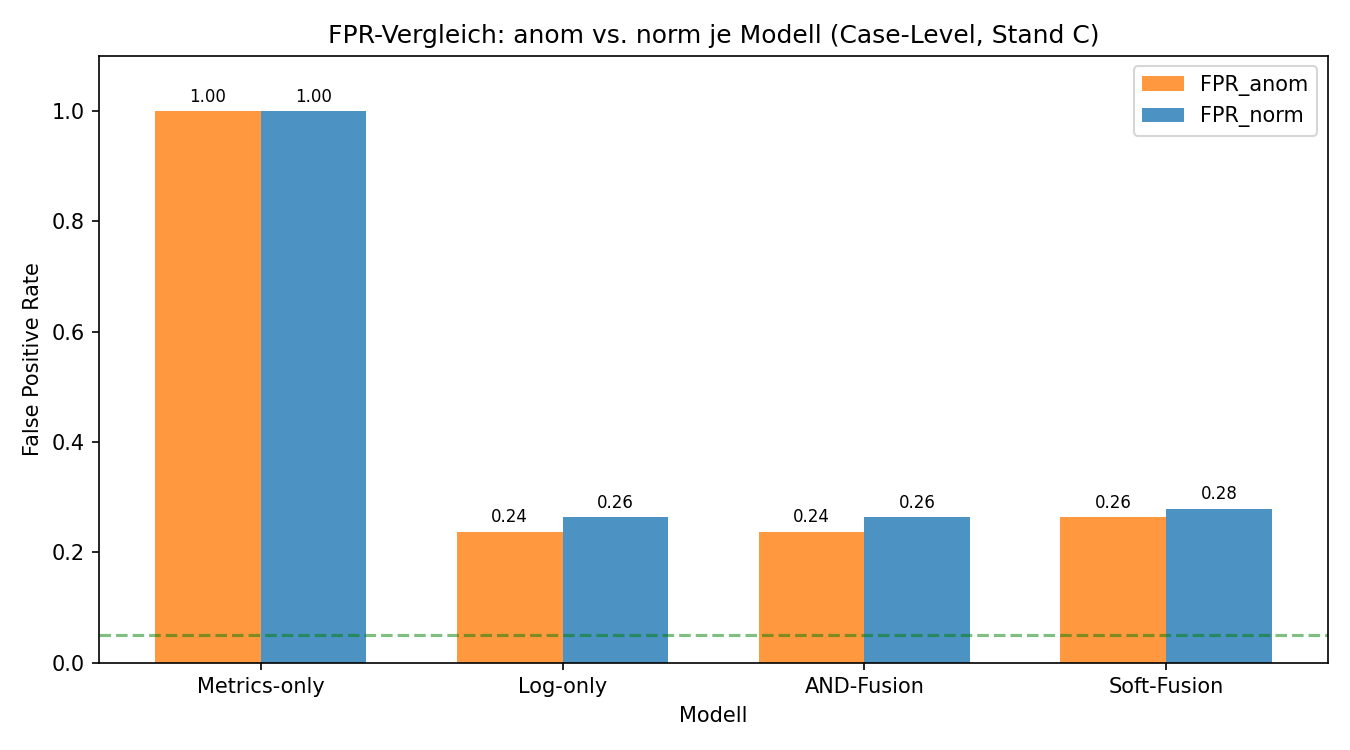
\includegraphics[width=0.82\textwidth]{../docs/fpr_comparison}
  \caption{Vergleich von $\mathrm{FPR}_{\mathrm{anom}}$ und $\mathrm{FPR}_{\mathrm{norm}}$ zwischen Metrik-Baseline, Log-Komponente und den beiden Fusionsvarianten (Case-Ebene, $n=253$).}
  \label{fig:fpr_comp}
\end{figure}

Die zentralen Befunde lassen sich wie folgt zusammenfassen: Metrics-only erkennt alle positiven Cases, klassifiziert aber alle negativen Cases als positiv (FPR$_{\text{total}}$ = 1{,}0000). Log-only ist die stärkste Variante mit FPR$_{\text{total}}$ = 0{,}2537 bei Recall$_{\text{mali}}$ = 0{,}9375 (AP = 0{,}6548). AND-Fusion degeneriert zu Log-only, da der metrische Trigger bei allen 253~Test-Cases aktiv ist (vgl. Abschnitt~\ref{sec:degeneration}). Soft-Fusion weist gegenüber Log-only denselben Recall auf, erzeugt jedoch zwei zusätzliche False Positives (54 vs.~52) und verschlechtert sich in Precision, F1, FPR und AP (F1: 0{,}6122 vs. 0{,}6207, FPR: 0{,}2634 vs. 0{,}2537, AP: 0{,}5553 vs. 0{,}6548). Soft-Fusion liefert daher keinen Zusatznutzen gegenüber Log-only. Auf diesem Benchmark liegt der wesentliche Beitrag zur False-Positive-Reduktion beim Log-Kontext. Die untersuchten Fusionsregeln liefern gegenüber Log-only keinen Mehrwert.

\subsection{Fehleranalyse auf Case-Ebene}
\label{sec:error_analysis}

Die folgenden Abschnitte analysieren qualitativ, welche Test-Cases von der Log-only-Komponente fehlklassifiziert werden. Diese Analyse stützt sich ausschließlich auf die bereits vorliegenden Test-Scores und -Trigger aus \texttt{docs/fusion\_cases.csv}. Es wurden keine Modelle neu trainiert, keine Thresholds verändert und keine testbasierte Optimierung durchgeführt.

\subsubsection{False-Negative-Cases}

Log-only verfehlt 3 von 48 positiven Test-Cases (Recall$_{\text{mali}}$ = 0{,}9375). Alle drei False Negatives entstammen derselben Gruppe (\texttt{mali/scenario\_6}, Szenarioname: \emph{Rootkit / Backdoor}) und liegen mit ihren Log-Scores moderat bis deutlich unterhalb des Validierungsthresholds $\tau_{\text{log}} = 0{,}1641$.

\begin{table}[htb]
  \centering
  \small
  \caption{False-Negative-Cases der Log-only-Komponente (Case-Ebene, Testset)}
  \label{tab:fn_cases}
  \begin{tabular}{lllp{6.2cm}}
    \hline
    \textbf{Case} & \textbf{Log-Score} & \textbf{Abstand zu $\tau$} & \textbf{Qualitative Beobachtung} \\
    \hline
    \texttt{mali\_6\_10} & 0{,}0719 & $-$0{,}0922 & Moderat unter Threshold, Treffer bei cron, sshd und root erkannt \\
    \texttt{mali\_6\_16} & 0{,}0671 & $-$0{,}0970 & Moderat unter Threshold, Treffer bei cron und sshd erkannt \\
    \texttt{mali\_6\_24} & 0{,}0553 & $-$0{,}1088 & Deutlich unter Threshold, Meldungen von cron und aide erkannt \\
    \hline
  \end{tabular}
\end{table}

Die Logs der drei Cases enthalten Treffer aus der vordefinierten Security-Keyword-Liste (\texttt{cron}, \texttt{sshd}, \texttt{root}, \texttt{/etc/}). Da Begriffe wie \texttt{cron} oder \texttt{sshd} in regulärem Systembetrieb generisch auftreten können, reichen diese Treffer im gewählten TF-IDF/LogReg-Modell nicht für eine positive Klassifikationsentscheidung aus. Die Fehleranalyse zeigt, dass \texttt{scenario\_6} (\emph{Rootkit / Backdoor}) ein Angriffsmuster enthält, dessen Log-Signatur vom Modell bei diesem Operating-Point nicht ausreichend erfasst wird.

Tabelle~\ref{tab:mali_scenario_recall} zeigt die Recall-Auf\-schlüs\-se\-lung nach malicious Test-Szenarien.\newline\texttt{scenario\_6} erreicht einen Recall von 0{,}8750 (21~von~24~Cases erkannt), während \texttt{scenario\_7} vollständig detektiert wird (Recall~=~1{,}0000). Das Szenario~6 ist damit insgesamt schwieriger, jedoch werden 21 von 24 Cases korrekt erkannt. Nur einzelne Cases liegen unterhalb der Entscheidungsgrenze, was auf eine uneinheitliche Log-Signatur innerhalb des Szenarios hindeutet.

\begin{table}[htb]
  \centering
  \caption{Malicious Test-Szenarien: Recall der Log-only-Komponente (aus \texttt{docs/mali\_test\_scenario\_recall.csv})}
  \label{tab:mali_scenario_recall}
  \begin{tabular}{llrrrr}
    \hline
    \textbf{Szenario} & \textbf{Name} & \textbf{n} & \textbf{TP} & \textbf{FN} & \textbf{Recall} \\
    \hline
    \texttt{mali/scenario\_6} & Rootkit / Backdoor & 24 & 21 & 3 & 0{,}8750 \\
    \texttt{mali/scenario\_7} & Brute-force / Credential Stuffing Attack & 24 & 24 & 0 & 1{,}0000 \\
    \hline
    \textbf{Gesamt} & & \textbf{48} & \textbf{45} & \textbf{3} & \textbf{0{,}9375} \\
    \hline
  \end{tabular}
\end{table}

Bei dem auf Validation ausgewählten Threshold bleiben die drei False-Negative-Cases unterhalb der Entscheidungsgrenze. Eine niedrigere Schwelle könnte den Recall erhöhen, würde jedoch voraussichtlich zusätzliche False Positives erzeugen. Dieser Trade-off wird in der Threshold-Sensitivity sichtbar (Abschnitt~\ref{sec:sensitivity}). Eine nachträgliche Anpassung auf Basis der Testmenge wäre methodisch nicht zulässig.

\subsubsection{False-Positive-Cases nach Szenario}

Die 52~False Positives von Log-only (FPR$_{\text{total}}$ = 0{,}2537) sind nicht gleichmäßig auf Szenarien verteilt. Tabelle~\ref{tab:fp_scenario} schlüsselt die Fehlklassifikationen für alle anom- und norm-Szenarien im Testset auf.

\begin{table}[htb]
  \centering
  \small
  \caption{False-Positive-Analyse nach Szenario für Log-only (Testset, 205 negative Cases)}
  \label{tab:fp_scenario}
  \begin{tabular}{llrrrr}
    \hline
    \textbf{Typ} & \textbf{Szenario} & \textbf{Cases} & \textbf{FP} & \textbf{FPR} & \textbf{$\bar{s}_{\text{log}}$} \\
    \hline
    anom & scenario\_17 & 18 & 11 & 0{,}6111 & 0{,}3218 \\
    anom & scenario\_5  & 30 &  6 & 0{,}2000 & 0{,}1405 \\
    anom & scenario\_13 & 28 &  1 & 0{,}0357 & 0{,}0937 \\
    norm & scenario\_8  & 30 & 30 & 1{,}0000 & 0{,}5226 \\
    norm & scenario\_15 & 30 &  2 & 0{,}0667 & 0{,}0861 \\
    norm & scenario\_6  & 24 &  1 & 0{,}0417 & 0{,}0717 \\
    norm & scenario\_4  & 45 &  1 & 0{,}0222 & 0{,}0534 \\
    \hline
    \multicolumn{6}{l}{\footnotesize FPR und $\bar{s}_{\text{log}}$ beziehen sich ausschließlich auf Log-only.} \\
  \end{tabular}
\end{table}

Die Fehleranalyse zeigt, dass die Fehlklassifikationen szenarioabhängig konzentriert sind. Im anom-Bereich dominiert \texttt{anom/scenario\_17} mit einer FPR von 0{,}6111 (11 von 18 Cases). Alle weiteren anom-Szenarien weisen deutlich niedrigere Raten auf. Für \texttt{anom/scenario\_17} liegt kein offiziell bekannter Szenarioname vor. Die Log-Scores dieses Szenarios liegen im Schnitt bei 0{,}3218 und damit weit oberhalb des Thresholds, was auf systematisch erhöhte Treffer aus der vordefinierten Security-Keyword-Liste hinweist, die das Modell stark mit mali-Klassen assoziiert.

Im norm-Bereich fällt \texttt{norm/scenario\_8} (\emph{Search Engine Aggressive Crawl}) besonders auf: Alle 30~norm-Cases des Szenarios werden positiv klassifiziert (FPR~=~1{,}0000, $\bar{s}_{\text{log}}$ = 0{,}5226). Ein aggressiver Web-Crawler erzeugt in Server-Logs oberflächlich attackenähnliche Muster, etwa dichte HTTP-Request-Serien, ungewöhnliche User-Agent-Strings oder wiederholte Zugriffsversuche, obwohl es sich um ein normales, wenn auch ressourcenintensives Ereignis handelt. Das TF-IDF-Modell kann diesen Unterschied allein anhand der Termstatistiken nicht zuverlässig auflösen. Dies erklärt, warum FPR$_{\text{norm}}$ = 0{,}2636 insgesamt etwas höher liegt als FPR$_{\text{anom}}$ = 0{,}2368. Eine kausale Erklärung der szenariospezifischen Log-Muster erfordert eine tiefere manuelle Log-Inspektion und liegt außerhalb des Kernumfangs dieser Arbeit.

\begin{figure}[htb]
  \centering
  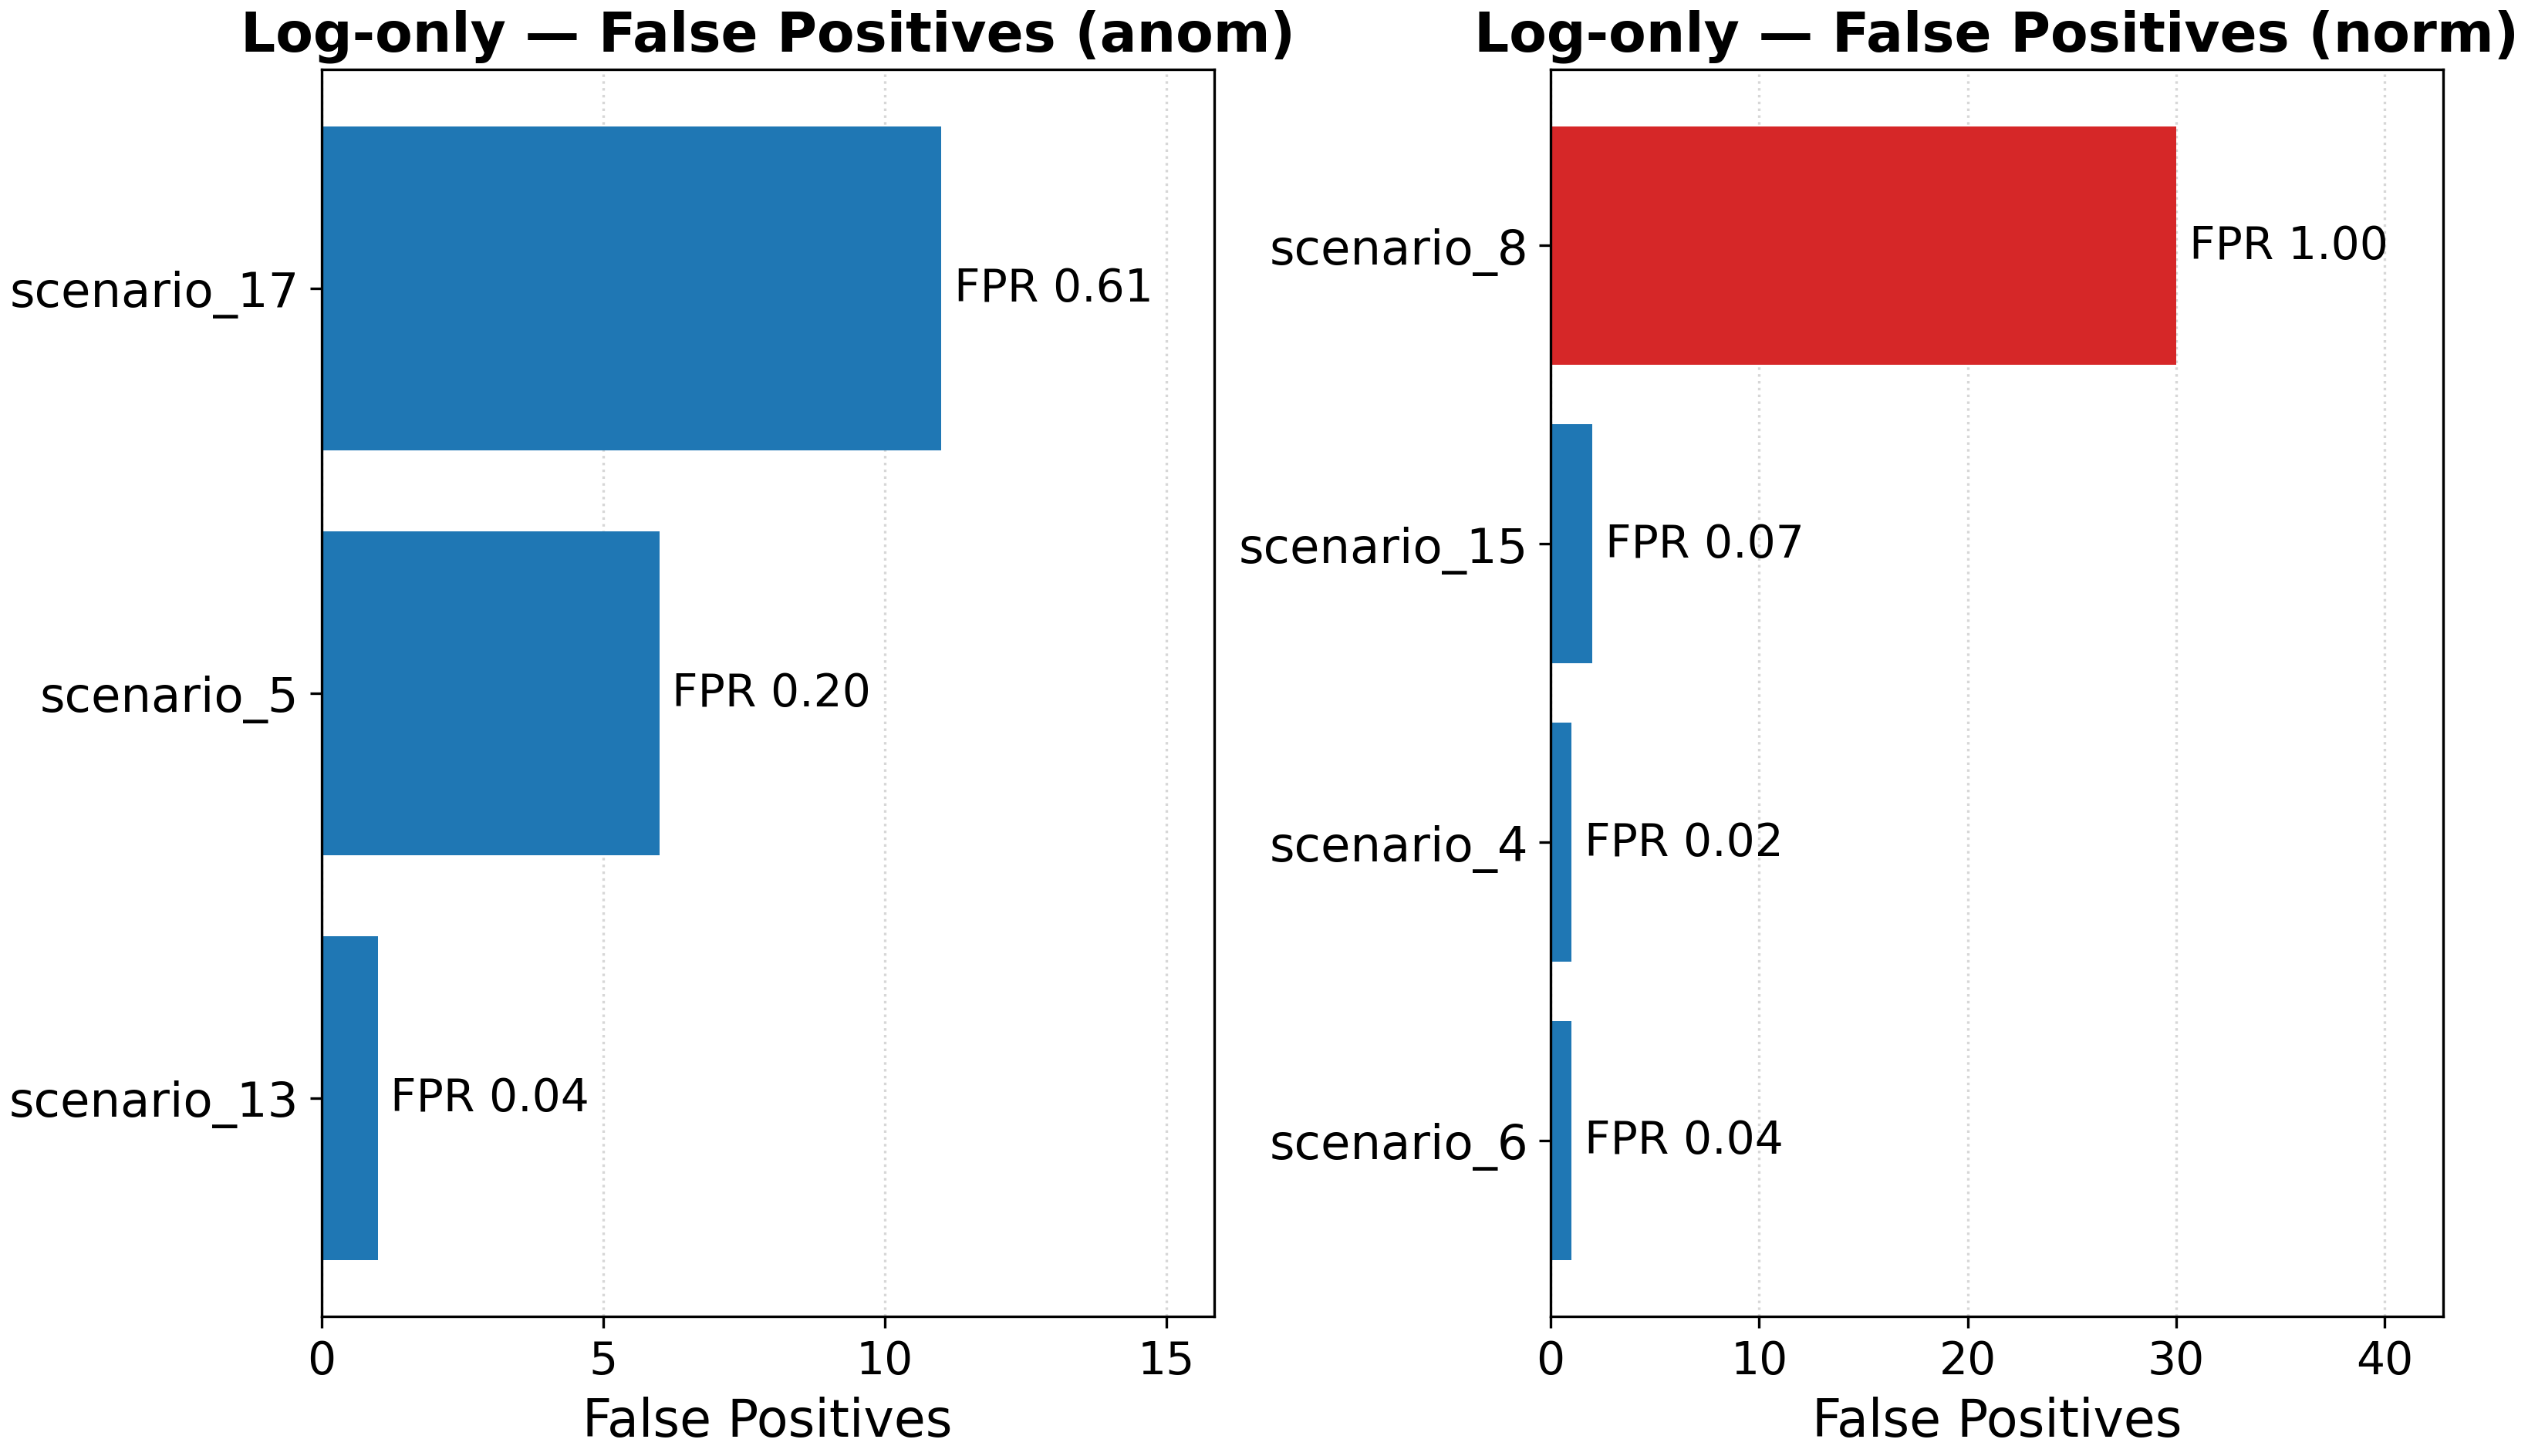
\includegraphics[width=\textwidth]{../docs/fp_by_scenario_logonly}
  \caption{False Positives nach Szenario für Log-only, aufgeschlüsselt nach anom (links) und norm (rechts). Die Annotation zeigt die szenariospezifische FPR. Rote Balken markieren Szenarien mit FPR~=~1{,}0.}
  \label{fig:fp_scenario}
\end{figure}

\subsection{AND-Gate-Degeneration}
\label{sec:degeneration}

Ein wesentlicher empirischer Befund dieser Arbeit ist die vollständige Degeneration des AND-Gates. Alle 253~Test-Cases erhalten ein \texttt{metric\_trigger=1} (253/253~=~100~\%). Kein einziger Case löst den Metrikdetektor nicht aus. Die AND-Fusion ist damit funktional identisch zur reinen Log-Filterung: Da die Bedingung \texttt{metric\_trigger=1} für jeden Case erfüllt ist, gilt $\texttt{AND} = \texttt{metric\_trigger} \wedge \texttt{log\_trigger} = \texttt{log\_trigger}$. Durch die Einbeziehung des Log-Kontexts sinkt die FPR gegenüber Metrics-only. Da der metrische Trigger jedoch alle Testfälle aktiviert, erzielt die AND-Fusion auf dem Testset keinen zusätzlichen Fusionsgewinn gegenüber Log-only. Die Konfusionsmatrizen von AND-Fusion und Log-only sind exakt gleich.

Die Ursache liegt in der Kalibrierung des Metrik-Detektors. Der niedrige Validierungsthreshold von~0{,}0258 markiert alle Test-Cases als metrisch auffällig, unabhängig von ihrer tatsächlichen Klasse. Die 25~Case-Level-Features der fünf universellen Metriken liefern auf diesem Benchmark keine ausreichende Trennkraft, um anom- und norm-Cases von mali-Cases zu unterscheiden. Viele technische Anomalien und Normalszenarien weisen ähnlich hohe Metrik-Aggregate wie Malware-Aktivitäten auf. Das AND-Gate, das konzeptionell als Zweistufenfilter gedacht ist, verliert dadurch seine Filterfunktion auf Metrikseite vollständig.

Diese Degeneration ist kein Implementierungsfehler, sondern ein direktes Ergebnis der Nicht-Selektivität des Metrik-Detektors auf Case-Ebene in diesem Benchmark. Sie muss bei der Interpretation der Ergebnisse transparent benannt werden. Eine Möglichkeit, die Degeneration zu überwinden, wäre der Einsatz eines ausdrucksstärkeren metrischen Detektors (z.\,B. mit typspezifischen Features oder anderen Modellklassen). Dies liegt außerhalb des Rahmens dieser Arbeit.

\subsection{Qualitätssicherung und Reproduzierbarkeit}

Die Kernlogiken der Pipeline werden durch 67~automatisierte Tests in 14~Klassen abgesichert (\texttt{test\_pipeline.py} im Verzeichnis \texttt{tests/}, pytest-Framework):

\begin{enumerate}
  \item \textbf{Canonical Matrix / Preprocessing} (\texttt{TestBuildCanonicalMatrix}, 4~Tests): Prüft die korrekte Behandlung fehlender Spalten, die Erhaltung von \texttt{NaN} vor dem Split, die vollständige NaN-Bereinigung nach evaluationsrelevanter Imputation sowie die Konvertierung von mit Anführungszeichen versehenen Zeichenketten.

  \item \textbf{Zeilen-Imputation} (\texttt{TestRowLevelImputation}, 6~Tests): Verifiziert, dass keine Medianimputation vor dem Split erfolgt, Imputationsmediane ausschließlich aus Trainingszeilen stammen, derselbe Median je Feature auf alle \texttt{dataset\_type}-Werte und Splits angewendet wird und die finalen 25~Case-Level-Features keine \texttt{NaN} enthalten.

  \item \textbf{Fusion / Soft-Score} (\texttt{TestFusionLogic}, 3~Tests): Verifiziert die AND-Gate-Wahr\-heits\-tabelle auf allen vier Eingangskombinationen sowie die Wertebereichseigenschaft des Soft-Scores ($s_{\text{fusion}} \in [0,1]$).

  \item \textbf{Datenintegrität / GroupShuffleSplit} (\texttt{TestDataIntegrity}, 2~Tests): Stellt sicher, dass keine Gruppe in mehr als einem der drei Splits gleichzeitig vorkommt, und prüft das Vorhandensein aller fünf universellen Features in sämtlichen Datensatztypen.

  \item \textbf{Algorithmische Logik} (\texttt{TestAlgorithmicLogic}, 4~Tests): Prüft die Threshold-Auswahllogik, die Recall-Nebenbedingung nach Threshold-Anwendung sowie die Abwesenheit testexklusiver Terme im TF-IDF-Vokabular.

  \item \textbf{Validierungs-Split} (\texttt{TestValidationSplit}, 6~Tests): Verifiziert die Disjunktheit aller drei Splits nach Gruppenkennung sowie die ausschließliche Verwendung von Trainingsdaten für Imputations-Mediane.

  \item \textbf{Threshold-Sensitivity} (\texttt{TestThresholdSensitivity}, 5~Tests): Prüft, dass die Sensitivity-Tabelle alle vier Recall-Ziele enthält, dass Thresholds ausschließlich aus Validierungsdaten stammen und dass Metriken im Einheitsintervall liegen.

  \item \textbf{Case-Level Metrik-Baseline} (\texttt{TestCaseLevelMetricBaseline}, 6~Tests): Verifiziert die Gruppendisjunktheit auf Case-Ebene, eine Zeile pro Case in den Feature-Artefakten, die Abwesenheit von Row-Level-Leakage in den Features sowie die validierungsbasierte Threshold-Wahl.

  \item \textbf{Log-Normalisierung und Scores} (\texttt{TestLogNormalizationAndScores}, 6~Tests): Prüft, dass die Normalisierungsfunktion IPs, Zeitstempel, PIDs und isolierte Zahlen ersetzt, sicherheitsrelevante Terme der vordefinierten Keyword-Liste erhält, Case-Level-Scores korrekt vorliegen und das TF-IDF-Vokabular ausschließlich auf Trainingsdaten gefittet wird.

  \item \textbf{Case-Level Fusion} (\texttt{TestCaseLevelFusion}, 7~Tests): Verifiziert, dass die Fusion ausschließlich Case-Level-Scores verwendet, eine Zeile pro Test-Case vorliegt, der Soft-Fusion-Threshold aus Validation stammt und die FPR-Aufschlüsselung nach Datensatztyp konsistent ist.

  \item \textbf{False-Negative-Analyse} (\texttt{TestFalseNegativeCases}, 3~Tests): Prüft, dass genau 3~FN-Cases vorliegen, alle dem Typ mali entstammen und ihre Log-Scores unterhalb des Validierungsthresholds liegen.

  \item \textbf{False-Positive-Szenario-Analyse} (\texttt{TestFalsePositiveByScenario}, 5~Tests): Verifiziert die szenariospezifische FP-Aggregation, die Konsistenz der FPR-Berechnung und die korrekte Identifikation der Top-Szenarien (\path{norm/scenario_8}, \path{anom/scenario_17}).

  \item \textbf{Fehleranalyse ändert keine Hauptergebnisse}\newline(\texttt{TestError\-Analysis\-DoesNot\-Change\-Final\-Results}, 1~Test): Stellt sicher, dass die diagnostische Fehleranalyse keine Modelle neu trainiert, keine Thresholds verändert und keine finalen Hauptmetriken beeinflusst.

  \item \textbf{Fresh-run-Determinismus} (\texttt{TestFreshRunSplitDeterminism}, 9~Tests): Verifiziert, dass die Split-Erzeugung keine bestehende \texttt{split\_assignments.csv} voraussetzt, gleiche Seeds bit-identische Zuordnungen liefern, alle drei Splits auf Case- und Gruppenebene disjunkt sind, Zeilenmediane ausschließlich aus Trainingszeilen stammen und der kanonische Split deterministisch reproduzierbar ist.
\end{enumerate}

Die Reproduzierbarkeit wird durch fixierte Zu\-falls\-seeds, gespeicherte Split-Zu\-ord\-nun\-gen,
eine dokumentierte Ausführungsreihenfolge, eine spezifizierte Umgebung, versionierte
Ergebnisartefakte und den finalen Repository-Commit unterstützt: Der finale Testsplit
verwendet \texttt{random\_state=42}. Der interne Validierungsanteil wird ohne Zugriff
auf das Testset über Seed~0 aus einer vordefinierten Kandidatenliste gewählt, sodass
ausreichend positive Validation-Cases enthalten sind. Das XGBoost-Training verwendet
ebenfalls \texttt{random\_state=42}. Die Datei \texttt{docs/fusion\_cases.csv} enthält
alle 253~Test-Cases mit ihren Zwischen-Scores (\texttt{metric\_score},
\texttt{log\_score}, \texttt{metric\_trigger}, \texttt{log\_trigger},
\texttt{and\_trigger}, \texttt{score\_fusion} und \texttt{soft\_fusion\_trigger}) als
nachvollziehbarer Audit-Trail.

% ---------------------------------------------------------------------------
\section{Diskussion und Limitationen}
% ---------------------------------------------------------------------------

\subsection{Beantwortung der Forschungsfrage}

Die Forschungsfrage lautete, ob eine zweistufige hybride Pipeline die False-Positive-Rate auf CloudAnoBench deutlich senken kann, ohne die Recall-Rate unter~0{,}95 zu drücken. Die Ablationsergebnisse in Abschnitt~\ref{sec:ablation} beantworten diese Frage differenziert: Die Log-Komponente reduziert die FPR$_{\text{total}}$ von 1{,}0000 (Metrics-only) auf 0{,}2537. Der Log-Kontext ist damit der bestimmende Faktor der False-Positive-Reduktion. Der Test-Recall$_{\text{mali}}$ beträgt 0{,}9375, was die angestrebte Schwelle von 0{,}95 knapp verfehlt (3~von~48~positiven Cases nicht detektiert). Die Fusionsstufe liefert keinen Zusatznutzen gegenüber Log-only.

Das entscheidende Systemelement ist die Log-Komponente. Die log-basierte Klassifikation auf Case-Ebene identifiziert anhand textueller Systemereignismuster, welche Cases nicht als malicious einzustufen sind. Die Fusionsstufe trägt in dieser Konfiguration keinen eigenständigen Beitrag: AND-Fusion degeneriert zu Log-only (metric\_trigger = 253/253~=~100~\%), und Soft-Fusion verschlechtert die Diskriminanz durch Multiplikation mit dem schwachen Metrik-Score.

\subsection{Rolle des Log-Kontexts}

Die deutliche FPR-Reduktion durch die Log-Komponente lässt sich durch den
zusätzlichen Informationsgehalt der Log-Daten erklären. Log-Meldungen enthalten
semantisch reichhaltige Ereignisbeschreibungen, die Ursache und Art eines
Betriebsvorgangs qualitativ charakterisieren können. Metriken hingegen messen quantitative Systemzustände und können zwischen unterschiedlichen Ereignistypen mit identischer Intensität nicht unterscheiden. TF-IDF kann diskriminierende Terme identifizieren, die in malignen Cases systematisch häufiger oder seltener auftreten als in normalen oder anomalen Cases~\cite{he2021survey}.

Die Analyse auf Case-Ebene statt Zeilenebene ist dabei konzeptuell angemessen: Die Entscheidung, ob ein Security-Alert ausgelöst werden soll, bezieht sich auf eine Beobachtungseinheit (Case) als Ganzes, nicht auf einen einzelnen Messpunkt.

\subsection{Grenzen der Metrik-Komponente}
\label{sec:limits_metric}

Der metrische Detektor erzielt mit einer AP von 0{,}2652 eine schwache Diskriminationsleistung auf Case-Ebene. Die Schema-Leakage-Vermeidung (vgl. Abschnitt~\ref{sec:features}) beschränkt das Modell auf 25~Case-Level-Features der fünf universellen Metriken (je Metrik: Mittelwert, Maximum, Standardabweichung, 95.~Perzentil, Trend). Diese Aggregate bieten keine ausreichende Trennkraft zwischen mali- und anom- und norm-Cases: Viele technische Anomalien und Normalszenarien erzeugen ähnlich hohe Metrik-Spitzen wie Malware-Aktivitäten. Die Konsequenz ist ein niedriger operativer Threshold von~0{,}0258, der alle 253~Test-Cases als metrisch auffällig markiert (FPR$_{\text{total}}$ = 1{,}0000, TN~=~0) und die vollständige Degeneration des AND-Gates bedingt.

Ein metrischer Detektor mit höherer Ausdrucksstärke, etwa durch typspezifische Features oder tiefere Modellklassen, könnte diese Einschränkungen möglicherweise mildern, ist jedoch mit dem Risiko erhöhten Schema-Leakages verbunden.

\subsection{Methodische Limitationen}
\label{sec:limit}

Mehrere methodische Einschränkungen begrenzen die Generalisierbarkeit der Befunde und müssen transparent benannt werden.

\textbf{Einzelner Train-/Validierungs-/Test-Split.} Es wurde lediglich ein einziger gruppenbasierter Train-/Validierungs-/Test-Split durchgeführt. Die Streuung der Ergebnismetriken über verschiedene Splits ist damit unbekannt. Threshold-Wahl und Early Stopping erfolgen ausschließlich auf dem Validierungsset, sodass das Testset als unberührter Holdout dient. Cawley und Talbot~\cite{cawley2010over} weisen darauf hin, dass die Abhängigkeit von einem einzigen Split die Stabilität der Ergebnisse nicht belegt. Bootstrap-Konfidenzintervalle oder wiederholte Splits könnten diese Limitation in zukünftigen Arbeiten adressieren.

\textbf{Kleine positive Testmenge.} Das Testset enthält lediglich 48~positive Cases (mali). Über das im Ausblick berichtete Wilson-Konfidenzintervall für den Recall hinaus wurden keine Konfidenzintervalle für die übrigen Metriken berechnet. Die Punktschätzungen der FPR und des Recalls sind daher mit entsprechender Vorsicht zu interpretieren.

\textbf{Begrenzte szenariospezifische Testabdeckung der mali-Klasse.} Der Testsplit enthält lediglich zwei malicious Szenarien (\texttt{mali/scenario\_6} und \texttt{mali/scenario\_7}). Der berichtete malicious Recall von~45/48 ist daher ein Befund auf diesem festen, scenario-aware Holdout-Split und darf nicht als empirische Abdeckung aller zwölf malicious Szenarien im Datensatz interpretiert werden. Der scenario-aware Split bleibt methodisch korrekt. Die Einschränkung betrifft allein die externe Breite der Recall-Aussage.

\textbf{Synthetischer Datensatz.} CloudAnoBench ist ein synthetisch generierter Datensatz und kein aufgezeichneter Produktions-Traffic. Ob die gelernten Textmuster auf andere Cloud-Umgebungen, andere Log-Formate oder reale Angriffe übertragbar sind, ist durch diese Arbeit nicht untersucht. Arp~et~al.~\cite{arp2022dos} weisen allgemein darauf hin, dass die Übertragbarkeit von im Labor evaluierten ML-Sicherheitsmodellen auf reale Einsatzumgebungen systematisch überschätzt werden kann.

\textbf{Einheitliche Case-Level-Evaluation.} In der finalen Pipeline werden Metrik-Baseline, Log-Komponente und Fusion auf derselben Granularität evaluiert: eine Zeile pro Case. Dadurch sind Recall, Precision, F1, AP sowie FPR$_{\text{total}}$, FPR$_{\text{anom}}$ und FPR$_{\text{norm}}$ direkt vergleichbar. Die Aussagekraft bleibt dennoch durch den einzelnen Holdout-Split begrenzt. Insbesondere beruhen die Recall-Werte im Testset auf 48 positiven mali-Cases.

\textbf{Recall-Gap der Log-Komponente.} Der Test-Recall der Log-Komponente verfehlt die angestrebte 0{,}95-Schwelle knapp. Die Threshold-Sensitivity-Analyse (vgl. Abschnitt~\ref{sec:sensitivity}) zeigt, dass keines der getesteten validierungsbasierten Recall-Ziele diesen Gap auf dem Testset schließt: Die betroffenen FN-Cases liegen unterhalb des niedrigsten Validierungsthresholds, der auf dem Validierungsset vollständigen Recall erzielt. Eine nachträgliche testbasierte Threshold-Optimierung wurde bewusst nicht durchgeführt, da sie dem Prinzip der leakage-sicheren Evaluation widerspräche~\cite{cawley2010over}.

\textbf{Soft-Fusion ohne Mehrwert gegenüber Log-only.} Die Soft-Fusion-Strategie ($s = \hat{p}_{\text{metric}} \times \hat{p}_{\text{log}}$) erzielt eine AP von~0{,}5553, die unter der AP der Log-Komponente allein (0{,}6548) liegt. F1 und FPR sind ebenfalls schlechter (F1: 0{,}6122 vs. 0{,}6207, FPR$_{\text{total}}$: 0{,}2634 vs. 0{,}2537). Die Ursache liegt darin, dass der metrische Score bei allen Test-Cases nahezu konstant hoch ist: Die Multiplikation nivelliert die Diskriminanz des Log-Scores, ohne einen eigenständigen Informationsgewinn zu liefern. Tax~et~al.~\cite{tax2000combining} zeigen, dass die Produktregel bei abhängigen oder redundanten Repräsentationen schlechter abschneiden kann. Eine alternative Fusionsgewichtung könnte diesen Nachteil möglicherweise beheben, wurde aber nicht untersucht.

\textbf{Prototypischer Implementierungscharakter.} Die gesamte Pipeline ist in Jupyter Notebooks implementiert und als Forschungsprototyp zu verstehen. Es existiert keine paketierte, produktionsreife Software-Implementierung.

\textbf{Keine tiefe manuelle Log-Inspektion einzelner norm-Cases.} Die Evaluation weist die FPR für norm-Cases (planmäßiger Betrieb, darunter Backup-Vorgänge und Batch-Jobs) separat aus. Für die beste Variante (Log-only) beträgt FPR\textsubscript{norm}~= 0{,}2636 (34~von~129~Cases). Eine tiefe manuelle Log-Inspektion einzelner falsch positiv klassifizierter norm-Cases wurde nicht durchgeführt. Die Zwischenergebnisse aller 253~Test-Cases, einschließlich metrischer und log-basierter Scores, sind in \texttt{docs/fusion\_cases.csv} dokumentiert und stehen für Anschlussanalysen bereit.

\subsection{Skalierbarkeit als konzeptuelle Einordnung}
\label{sec:scalability}

Konzeptuell ließe sich die Pipeline als verteilbare Abfolge von Filter- und Verifikationsschritten auffassen, etwa in Form einer Map/Reduce-artigen Aufteilung: Die metrische Vorab-Filterung (Phase~2) lässt sich als parallele Map-Operation auf Case-Ebene interpretieren, die log-basierte Verifikation (Phase~3) als fallweise Klassifikation auf dem normalisierten Log-Text.

Es ist jedoch ausdrücklich festzuhalten, dass diese Skalierbarkeitsbetrachtung konzeptueller Natur ist. Eine verteilte Implementierung wurde im Rahmen dieser Arbeit weder realisiert noch gemessen. Die gemessenen Laufzeiten der einzelnen Notebook-Phasen sind als indikative Einzelmessungen zu verstehen und hängen von Ausführungskontext, Hardware und Notebook-Umgebung ab. Sie werden daher nicht als belastbarer Benchmark herangezogen. Für die Bewertung dieser Arbeit entscheidend ist allein die konzeptuelle Zerlegung der Pipeline in getrennte, grundsätzlich parallelisierbare Schritte.

Eine Einbettung der Pipeline in Data-Intelligence-Plattformen wie Databricks oder Snowflake sowie ein automatisiertes Modell-Lifecycle-Management, etwa über MLflow zur Überwachung von Model~Drift in dynami\-schen Cloud-Um\-gebungen, wären naheliegende Erweiterungen für eine produktionsnahe Umsetzung. Diese Aspekte wurden in der vorliegenden Arbeit weder implementiert noch empirisch evaluiert und liegen außerhalb des Rahmens dieser Benchmark-Studie. Die Skalierbarkeitsbetrachtung bleibt daher auf die konzeptuelle Zerlegung der Pipeline in verteilbare Filter- und Verifikationsschritte beschränkt.

% !TeX encoding = UTF-8
% !TeX root = thesis.tex

\section{Fazit und Ausblick}

% ---------------------------------------------------------------------------
\subsection{Zusammenfassung}
% ---------------------------------------------------------------------------

Diese Arbeit hat eine zweistufige hybride Pipeline zur Reduzierung von
False Positives in der Cloud-Anomalieerkennung entwickelt und auf dem
synthetischen Benchmark CloudAnoBench evaluiert. Der methodische Fokus lag
auf einer leakage-sicheren Evaluation unter einer festen
Recall-Nebenbedingung ($R \geq 0{,}95$), nicht auf der Maximierung
einzelner Metriken. Beide Komponenten~--- metrischer Detektor und
Log-Verifikation~--- wurden isoliert und in zwei Fusionskonfigurationen
evaluiert; alle Ergebnisse sind durch einen festen Zufallszustand und
13~Unit-Tests reproduzierbar.

% ---------------------------------------------------------------------------
\subsection{Beantwortung der Forschungsfrage}
% ---------------------------------------------------------------------------

Die Forschungsfrage wird bejaht: Die Log-Komponente reduziert die FPR von
$79{,}8\,\%$ auf $26{,}3\,\%$ bei einem Recall von $0{,}958$~--- die
Recall-Nebenbedingung ist damit erfüllt. Die vollständige Ergebnisanalyse
und Argumentation findet sich in Abschnitt~\ref{sec:ablation} und den
Abschnitten zur Diskussion.

Der qualifizierende Befund ist, dass Log-Kontext auf Case-Ebene als
eigenständiger Prädiktor dominiert und die Fusionsstufe keinen zusätzlichen
Beitrag liefert: Das AND-Gate verliert aufgrund des niedrigen
Metrik-Thresholds seine Filterfunktion auf Metrikseite; die Soft-Fusion
erzielt eine niedrigere AP als die Log-Komponente allein. Die Nützlichkeit
einer AND-Fusion hängt damit entscheidend von der Kalibrierung des
Metrik-Triggers auf Case-Ebene ab, die in dieser Arbeit nicht umgesetzt wurde.

Diese Befunde gelten für den CloudAnoBench-Datensatz unter den gewählten
Konfigurationen und sind ohne weitere Evidenz nicht zu verallgemeinern.

% ---------------------------------------------------------------------------
\subsection{Ausblick}
% ---------------------------------------------------------------------------

Aus den Befunden dieser Arbeit ergeben sich mehrere konkrete Ansatzpunkte
für zukünftige Arbeiten:

\begin{description}
  \item[Case-Level-Kalibrierung des Metrik-Triggers.]
    Die AND-Gate-Degeneration ist eine direkte Folge der Threshold-Wahl auf
    Zeilenebene. Eine Kalibrierung direkt auf aggregierten Case-Scores~---
    oder der Einsatz alternativer Aggregationsregeln wie Median statt
    Maximum~--- würde die AND-Gate-Logik erst operativ wirksam machen und
    den eigenständigen Beitrag der Metrik-Komponente zur Fusion prüfbar machen.

  \item[Alternative Fusionsregeln.]
    Neben AND-Gate und Produkt-Regel existieren weitere Fusionsstrategien~---
    etwa Summen-Regel, gewichtete Mehrheitsentscheidung oder lernbasierte
    Kombinatoren. Ob solche Regeln auf CloudAnoBench einen messbaren Vorteil
    gegenüber der Log-Komponente allein erzielen, bleibt eine offene Frage.

  \item[Weiterentwicklung der Log-Komponente.]
    Die log-basierte Verifikation wurde in dieser Arbeit als interpretierbare
    Baseline mit TF-IDF und logistischer Regression umgesetzt. Ob
    struktur-bewusste Log-Parser, vortrainierte Sprachmodelle oder
    Embedding-Methoden auf diesem Datensatz zu einer weiteren FPR-Reduktion
    führen, wäre eine naheliegende Erweiterung.

  \item[Statistische Absicherung.]
    Die berichteten Metriken basieren auf einem einzigen Trainings"=Test"=Split.
    Die Frage, wie stabil die Ergebnisse über verschiedene Splits sind, ließe
    sich durch Bootstrap-Konfidenzintervalle oder wiederholte Splits mit
    unterschiedlichen Zufallszuständen beantworten.

  \item[Evaluation auf realem Produktions-Traffic.]
    CloudAnoBench verwendet kontrollierte Anomalie-Injektionen. Ob die
    gelernten Muster auf reale Infrastrukturdaten~--- mit natürlichen
    Klassenverteilungen, variablen Log-Formaten und unbekannten
    Anomalietypen~--- übertragbar sind, ist durch diese Arbeit nicht
    untersucht und stellt eine wichtige Anschlussfrage dar.

  \item[Modularisierung der Pipeline.]
    Die funktionale Pipeline liegt derzeit überwiegend in Jupyter Notebooks.
    Eine Modularisierung in eine paketierbare, konfigurierbare
    Software-Pipeline würde die Wiederverwendbarkeit und Anpassbarkeit an
    andere Datensätze wesentlich verbessern.
\end{description}


\printbibliography

\appendix
% !TeX encoding = UTF-8
% !TeX root = thesis.tex

\section{Anhang}

Die zur Reproduktion relevanten Artefakte befinden sich im Repository: die vier
Jupyter-Notebooks (\texttt{01\_data\_exploration}, \texttt{02\_metric\_baseline},
\texttt{03\_log\_component}, \texttt{04\_fusion}), die erzeugten Abbildungen
im Verzeichnis \texttt{docs/} sowie die 13~Unit-Tests in
\texttt{tests/test\_pipeline.py}.

Ergänzend liegt im Repository ein \texttt{Dockerfile} vor, das eine einfache
Jupyter-Lab-Umgebung auf Basis von Python~3.12 mit den benötigten Abhängigkeiten
bereitstellt. Es dient der lokalen Reproduzierbarkeit der Notebook-Ausführung und
ist nicht als produktionsreife Deployment-Umgebung zu verstehen. Der Container kann
aus dem Repository-Wurzelverzeichnis mit
\texttt{docker build -t cloudanobench-thesis .}
gebaut und anschließend mit
\texttt{docker run -p 8888:8888 cloudanobench-thesis}
gestartet werden.


\end{document}
